\documentclass[11pt,handout,xcolor=pdftex,dvipsnames,table,mathserif,aspectratio=169]{beamer}
\usetheme{metropolis}
%\usetheme{Darmstadt}
%\usepackage{times}
%\usefonttheme{structurebold}

\usepackage[english]{babel}
%\usepackage[table]{xcolor}
\usepackage{amsmath}
\usepackage{pgf,pgfarrows,pgfnodes,pgfautomata,pgfheaps}
\usepackage{amsmath,amssymb,setspace}
\usepackage[latin1]{inputenc}
\usepackage[T1]{fontenc}
\usepackage{relsize}

%\usepackage{pxfonts}

\usepackage[absolute,overlay]{textpos} 
\newenvironment{reference}[2]{% 
  \begin{textblock*}{\textwidth}(#1,#2) 
      \footnotesize\it\bgroup\color{red!50!black}}{\egroup\end{textblock*}} 

\DeclareMathSizes{10}{10}{6}{6} 


\title [Nonparametrics]{Nonparametrics and Local Methods}
\author{C.Conlon}
\institute{Applied Econometrics}
\date{\today}
\setbeamerfont{equation}{size=\tiny}
\begin{document}

\begin{frame}
\titlepage
\end{frame}



\begin{frame}{Basic Non-parametrics}
We all are familiar with models like this:
\begin{eqnarray*}
E[Y_i | X_i ] = \beta_0 + \beta_1 X_1 + \ldots 
\end{eqnarray*}
\begin{itemize}
\item Why is the conditional expectation function linear? Does it need to be?
\item Plenty of real-world phenomenon are nonlinear.
\item We can do things like this:
\begin{eqnarray*}
\log y_i = \beta_0 + \beta_1 X_1 + \beta_2 X^2 + \ldots + \varepsilon_i
\end{eqnarray*}
\item But this still a \alert{linear model}. Why?
\end{itemize}
\end{frame}

\begin{frame}{Basic Non-parametrics}
We've seen some other examples:
\begin{align*}
Y_{i} &= 1 \quad \mbox{if } Y_i^* >0\\
Y_{i} &= 1 \quad \mbox{if } Y_i^* \leq 0\\
Y_i^* &= \beta_0 + \beta_1 X_{1i} + \ldots + \varepsilon_i \quad \varepsilon_i \sim N (0,\sigma^2)
\end{align*}
\begin{itemize}
\item The probit estimator is a nonlinear function of its parameters.
\end{itemize}
\end{frame}


\begin{frame}{How about logit?}
We've seen some other examples:
\begin{align*}
Y_{i} &= 1 \quad \mbox{if } Y_i^* >0\\
Y_{i} &= 1 \quad \mbox{if } Y_i^* \leq 0\\
Y_i^* &= \beta_0 + \beta_1 X_{1i} + \ldots + \varepsilon_i \quad \varepsilon_i \sim Type I EV / Gumbel
\end{align*}
This is not how we usually write things
\end{frame}

\begin{frame}{How about logit?}
Instead we usually write:
\begin{align*}
E[Y_i | X_i] &= Pr(Y_i =1 | X_i) = p(x_i)\\
 Pr(Y_i =1 | X_i)  &= \frac{1}{1+\exp^{\beta_0 + \beta_1 x_1 + \beta_2 x_2 + \ldots}}
\end{align*}
Or with the log odds transformation:
\begin{align*}
\log \left(\frac{p}{1-p} \right) =\beta_0 + \beta_1 x_1 + \beta_2 x_2 + \ldots
\end{align*}
Logit is \alert{linear} again (in parameters). This is a \alert{generalized linear model}.
\end{frame}

\begin{frame}{How else might we estimate $E[Y_i | X_i]$?}
Obvious approach:
\begin{itemize}
\item With enough data: look at all values for $X_i = x$ and take the mean.
\item Easy if $X$ is discrete or doesn't take on too many values (Gender, State/Country).
\item Could work if $X$ is continuous but rounded (test scores, years of school, etc.).
\item We could cut $x_i$ into distinct bins (like a histogram).
\end{itemize}
\end{frame}


\begin{frame}{A Fake Data Example}
Following the THF textbook example, we can generate some fake data and let: 
\begin{eqnarray*}
Y=&ORANGE \mbox{ if } Y* &> 0.5 \\
Y=&BLUE  \mbox{ if }   Y* &\leq 0.5
\end{eqnarray*}
\begin{itemize}
\item Easiest way to recover $Y*$ is by running OLS on the linear probability model.
\item Draws from bivariate normal distribution with uncorrelated components but different means (2 overlapping types)
\item Mixture of 10 low variance (nearly point mass) normal distributions where the individual means were drawn from another normal distribution. (10 nearly distinct types).
\end{itemize}
\end{frame}

\begin{frame}{Linear Probability Model}
\begin{figure}[htbp]
\begin{center}
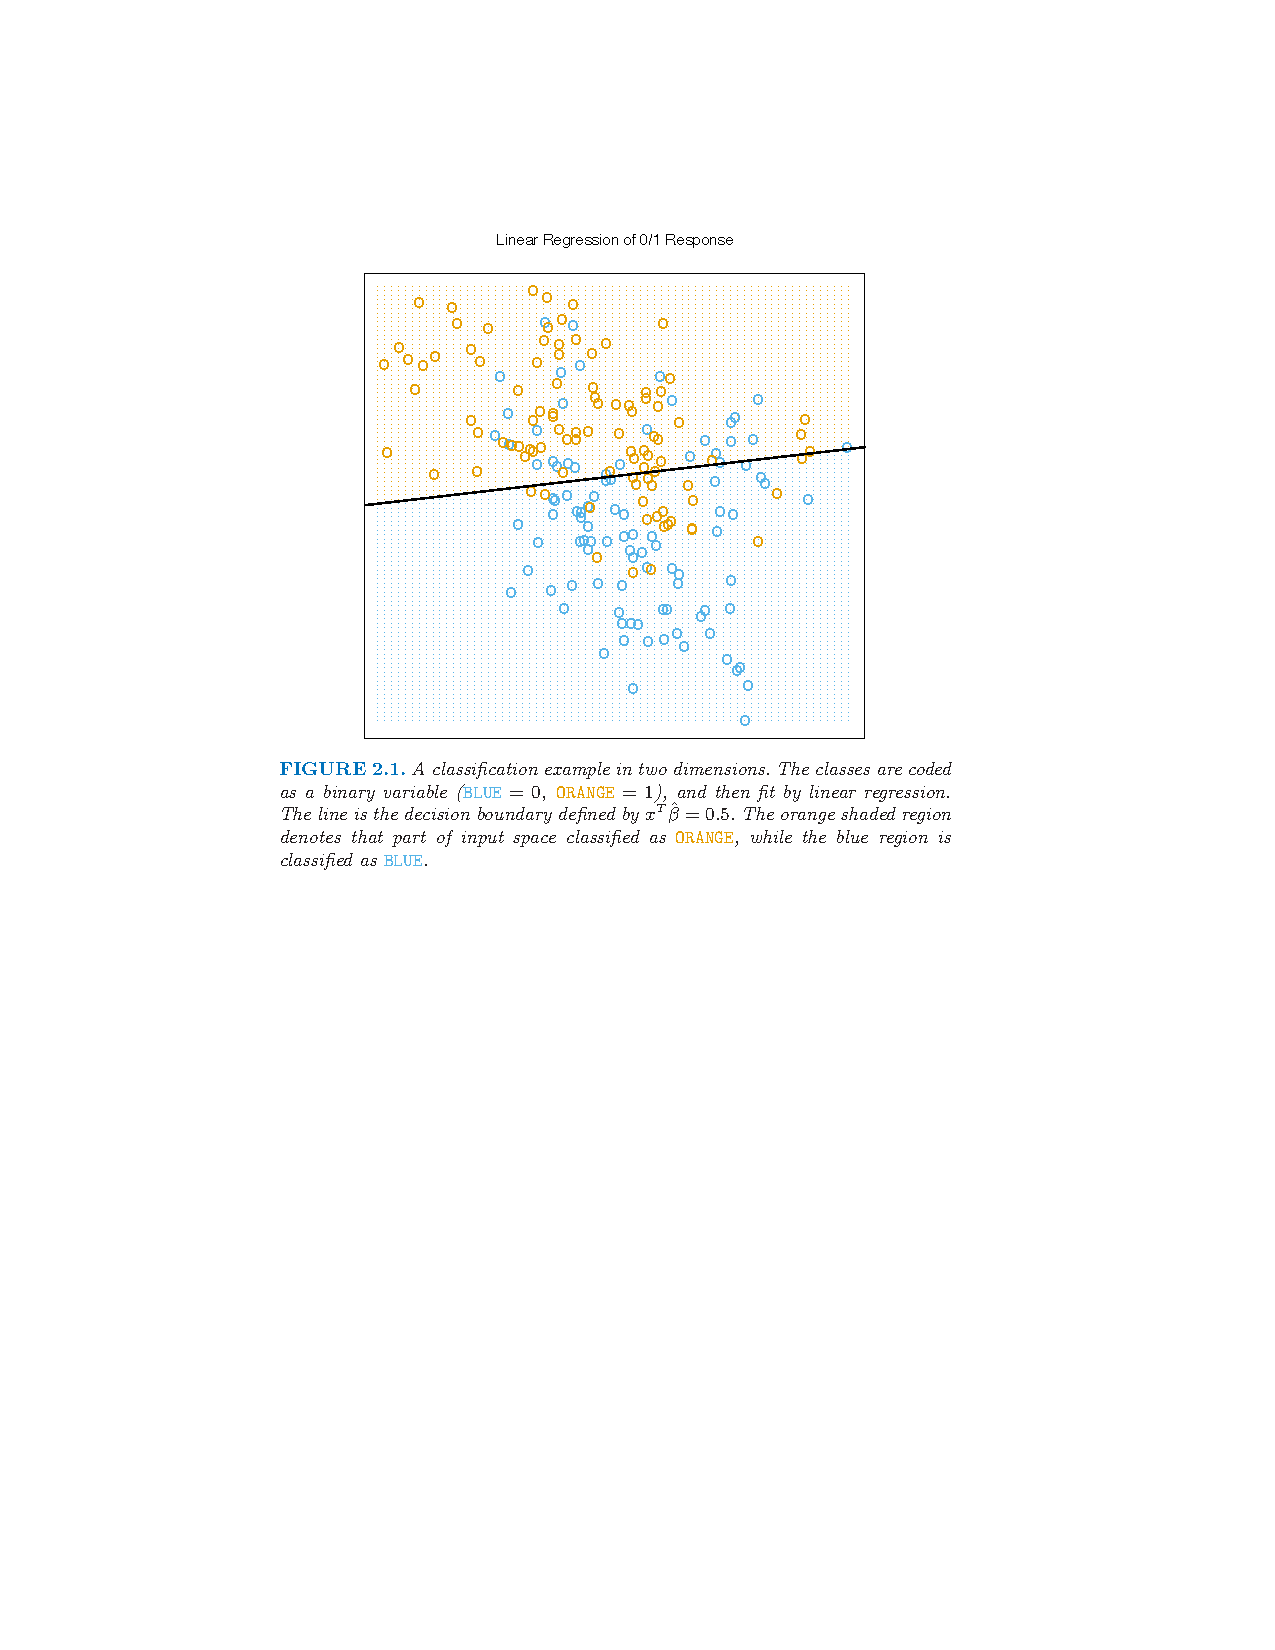
\includegraphics[width=3.5in]{./resources/classifierOLS.pdf}
\label{classOLS}
\end{center}
\end{figure}
\end{frame}


\begin{frame}{Alternative}
\begin{itemize}
\item Lots of potential alternatives to our decision rule.
\item A simple idea is to hold a majority vote of neighboring points 
\begin{eqnarray*}
Y^{*} = \frac{1}{k} \sum_{x_i \in N_k(x)} y_i
\end{eqnarray*}
\item To avoid including ``yourself'' in your neighborhood, we often estimate on one sample and validate on another
\item How many parameters does this model have: None? One? $k$? 
\item Technically it has something like $N/k$.
\item As $N \rightarrow \infty$ this means we have an infinite number of parameters! (This is a defining characteristic of non-parametrics).
\end{itemize}
\end{frame}


\begin{frame}{15 Nearest Neighbor}
\begin{figure}[htbp]
\begin{center}
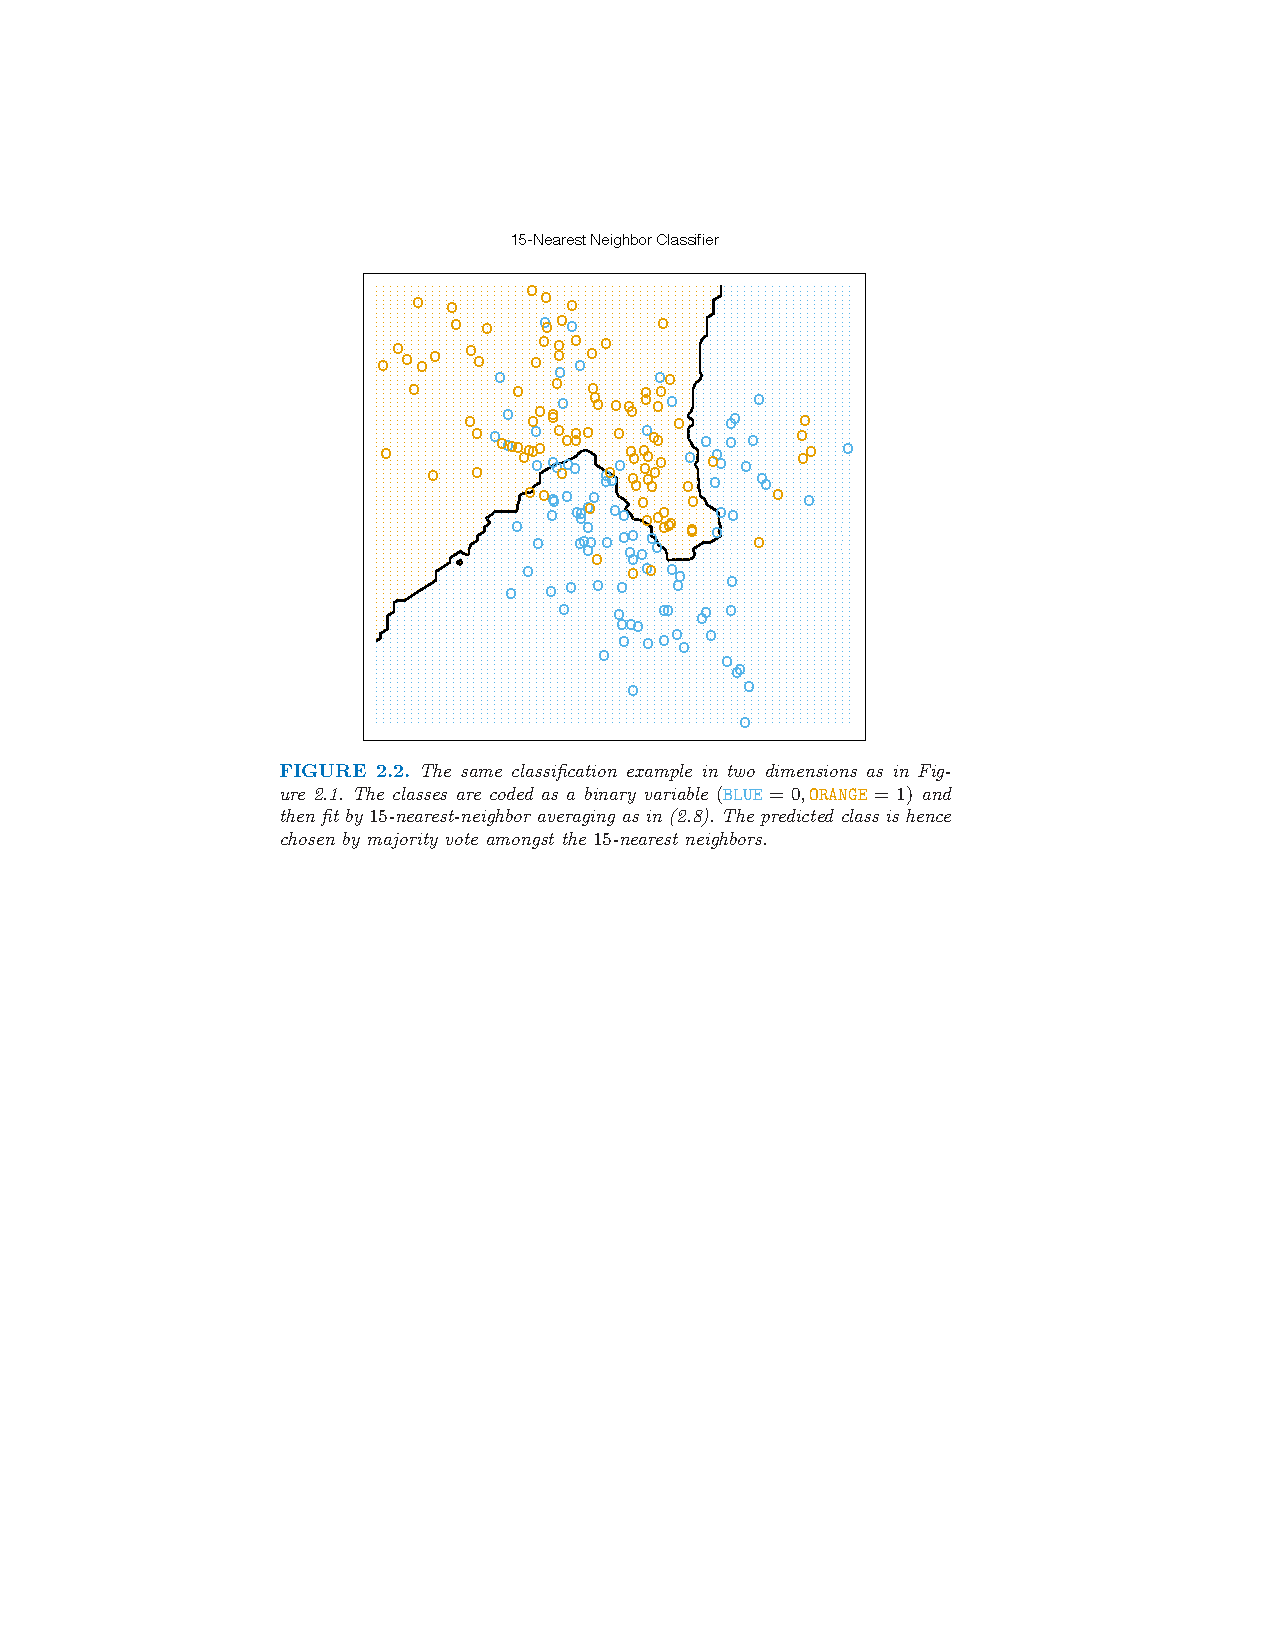
\includegraphics[width=3.5in]{./resources/classifier15nn.pdf}
\label{class15nn}
\end{center}
\end{figure}
\end{frame}

\begin{frame}{Extreme: 1 Nearest Neighbor}
\begin{figure}[htbp]
\begin{center}
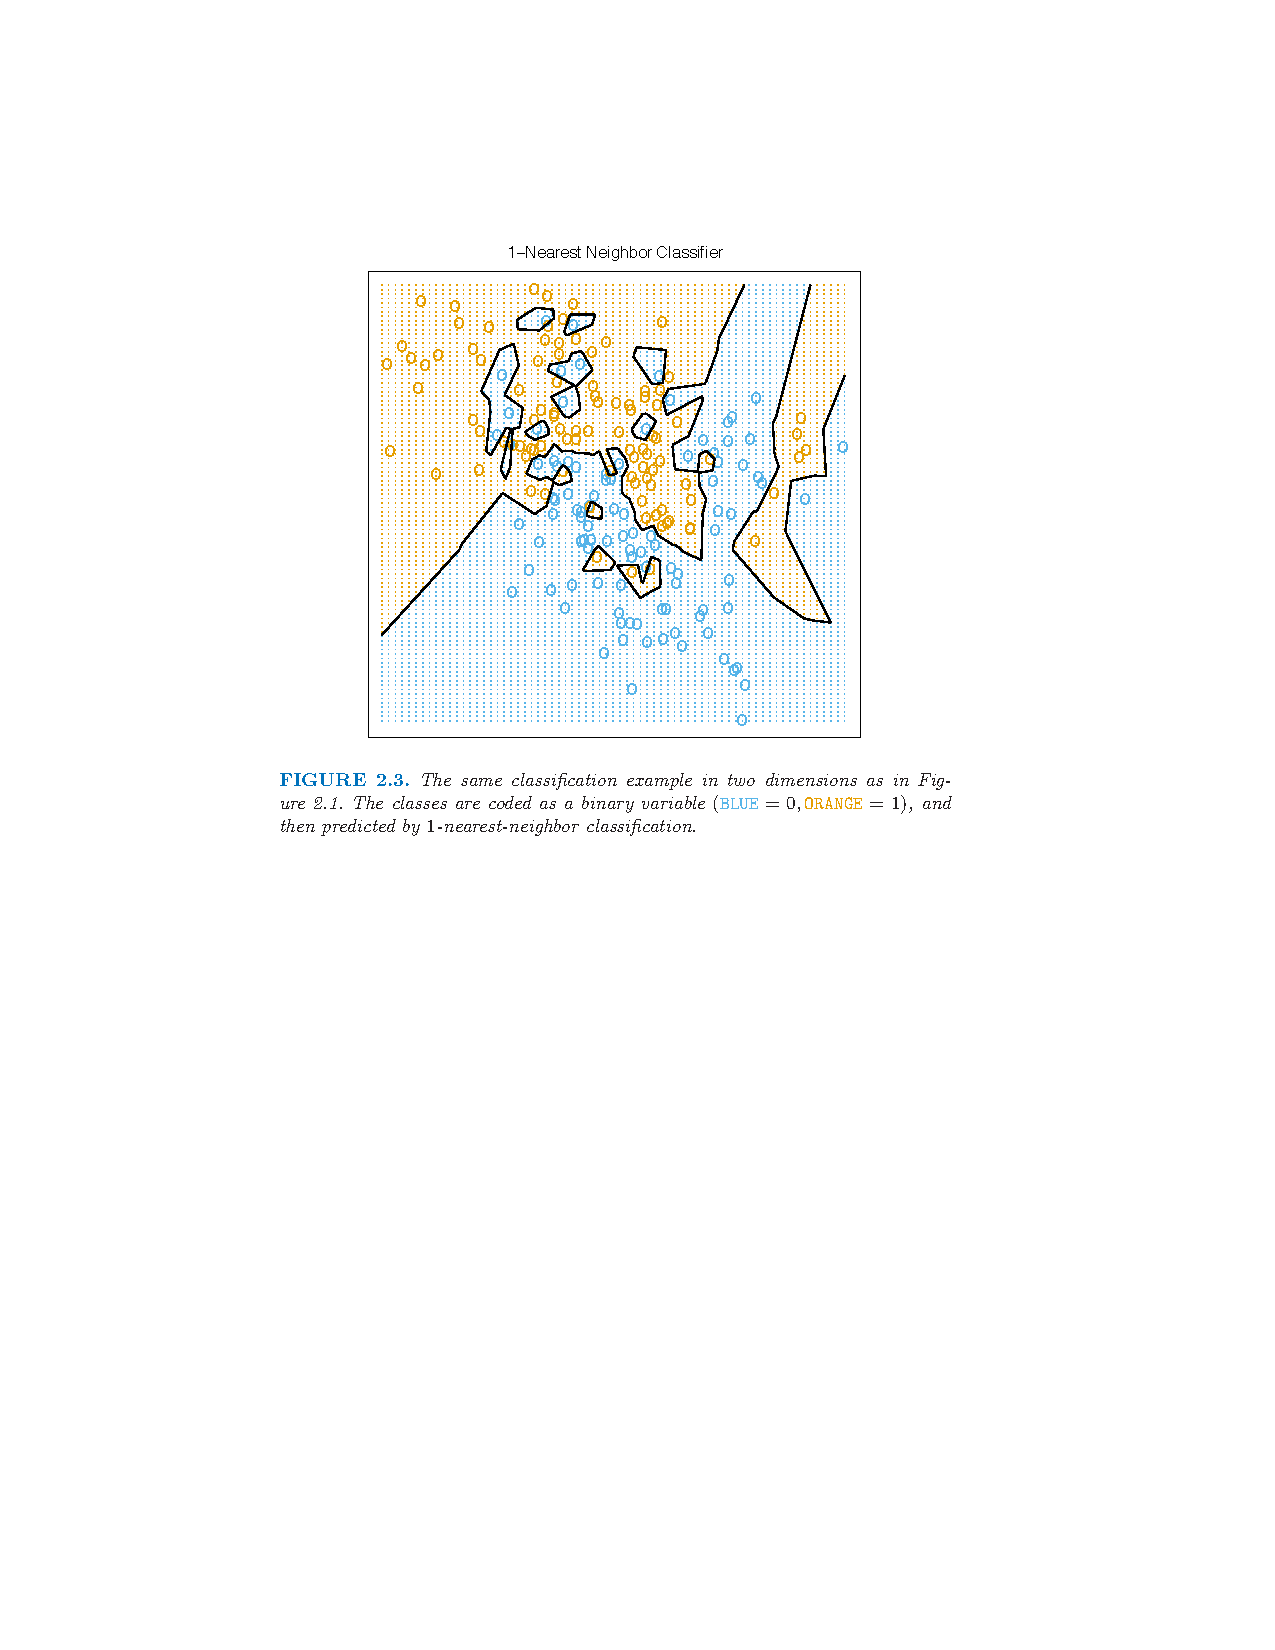
\includegraphics[width=3.5in]{./resources/classifier1nn.pdf}
\label{class15nn}
\end{center}
\end{figure}
\end{frame}

\begin{frame}{Comparisons}
\begin{itemize}
\item What would happen if $K \rightarrow N$?
\item The k-NN model is locally constant.
\item The k-NN approach tends to be really bumpy which can be undesirable.
\item The OLS model is globally linear (is this always true?)
\end{itemize}
\end{frame}
\begin{frame}{What about?}
\begin{itemize}
\item If we fixed the fact that there are discrete jumps in who is in the neighborhood by smoothly weighting observations and varying those weights instead (Kernels).
\item Another drawback of $k-NN$ is that we consider distance in each $X$ dimension on the same scale, perhaps we could rescale the data to improve our ``closeness'' measure.
\item Instead of fitting a constant locally, we fit a linear function locally (Lowess).
\item Instead of using a global linear approximation in OLS use a more flexible nonlinear one.
\item There is a bias/variance tradeoff. \alert{explain}.
\end{itemize}
\end{frame}

\begin{frame}{Bias Variance Decomposition}
We can decompose any estimator into two components
\begin{eqnarray*}
\underbrace{E[(y- \hat{f}(x))^2]}_{MSE} =\underbrace{\left( E[\hat{f}(x) - f(x)] \right)^2}_{Bias^2}  +  \underbrace{E \left[ \left(\hat{f}(x) - E[\hat{f}(x) \right] \right)^2}_{Variance} 
\end{eqnarray*}
\begin{itemize}
\item In general we face a tradeoff between bias and variance.
\item In k-NN as $k$ gets large we reduce the variance (each point has less influence) but we increase the bias since we start incorporating far away and potentially irrelevant information.
\item In OLS we minimize the variance among unbiased estimators assuming that the true $f$ is linear.
\end{itemize}
\end{frame}

\begin{frame}{Bias Variance Decomposition}
What minimizes MSE?
\begin{eqnarray*}
f(x_i) = E[Y_i | X_i] 
\end{eqnarray*}
\begin{itemize}
\item Seems simple enough (but we are back where we started).
\item How do we compute the expectation ?
\item k-NN tries to use local information to estimate conditional mean
\item OLS uses entire dataset and adds structure $ y = x \beta$ to the problem.
\end{itemize}
\end{frame}




\begin{frame}{Something Familiar}
Let's start with something we all know, how to calculate:
\begin{eqnarray*}
E[Y_i | X_i ] = \beta_0 + \beta_1 X_1 + \ldots + \varepsilon_i
\end{eqnarray*}
\begin{itemize}
\item The Gauss-Markov theorem (remember that?) tells us that OLS is best among linear unbiased estimators.
\end{itemize}
\end{frame}
%
%\begin{frame}{Identification}
%What does it mean for a model to be identified?
%\begin{eqnarray*}
%\hat{\beta}_{OLS} = \arg \max_{\beta} (\mathbf{y} - \mathbf{x} \beta)' (\mathbf{y} - \mathbf{x} \beta)
%\end{eqnarray*}
%\begin{itemize}
%\item We need there to be a unique value of $\beta$ that solves the above equation.
%\item For OLS this reduces to solving a linear system of $\dim(X)=k$ equations and unknowns.
%\item The OLS estimator produces $\hat{\beta}_{OLS} = \beta + (X'X)^{-1}X'\varepsilon$.
%\begin{itemize}
%\item Identification: means that we require $(X'X)$ is invertible (no perfect multicollinearity).
%\item When $E[X' \varepsilon ] =0$ then this converges in probability to true $\beta$.
%\end{itemize}
%
%\end{itemize}
%\end{frame}
%
%\begin{frame}{A Little More Complicated}
%\begin{itemize}
%\item For many cases that we care about, $E[X' \varepsilon ] \neq 0$. (Endogeneity)
%\item We know this is not the end of the world if we have an instrument $Z$:
%\item Now we need that $Z'X$ is invertible.
%\end{itemize}
%\begin{eqnarray*}
%E[\mathbf{x}' (\mathbf{y} - \mathbf{x} \beta)] &\neq& 0\\
%E[\mathbf{z}' (\mathbf{y} - \mathbf{x} \beta)] &=&0\\
%\rightarrow \hat{\beta}_{TSLS} &=& E(Z'X)^{-1} E[Z'Y]
%\end{eqnarray*}
%\end{frame}
%
%
%\begin{frame}{Some more information}
%This leads to the common terminology:
%\begin{itemize}
%\item Under-identified: if $\dim(X) > \dim(Z)$.
%\item Just-identified: if $\dim(X) = \dim(Z)$.
%\item Over-identified: if $\dim(X) < \dim(Z)$.
%\end{itemize}
%\end{frame}
%
%\begin{frame}{What does this mean exactly}
%To understand this we usually construct the GMM form of the moment conditions:
%\begin{eqnarray*}
%E[\mathbf{z}' (\mathbf{y} - \mathbf{x} \beta)] &=&0\\
%f(\beta)&=&  (\mathbf{y} - \mathbf{x} \beta)' \mathbf{z} \cdot W \cdot \mathbf{z}' (\mathbf{y} - \mathbf{x} \beta)
%\end{eqnarray*}
%\begin{itemize}
%\item Because $f(\beta)$ is a quadratic form, and when $W$ is PSD then $f(\beta) \geq 0$.
%\item Just-identified: There is exactly one solution to $f(\beta) = 0$ which does not depend on $W$.
%\item Under-identified: $f(\beta) = 0$ has many solutions because we have fewer instruments (or moment restrictions) than parameters.
%\item Over-identified: There are no solutions and $f(\beta) > 0$. Instead we choose $\beta$ to minimize the distance from zero with distance metric $W$.
%\end{itemize}
%\end{frame}
%
\begin{frame}{The Binary Case}
Now let's think about a case where $Y \in \{0,1\}$:
\begin{eqnarray*}
y_i = \mathbf{1}[F(X_i) - \varepsilon_i > 0]
\end{eqnarray*}
\begin{itemize}
\item There are different choices of $F(X_i)$ and $f(\varepsilon)$
\item  Probit: $F(X_i) = \beta X_i$ where $\varepsilon_i \sim N(0,1)$.
\item  Logit: same $F(\cdot)$ but different $f(\varepsilon)$ (Type I Extreme Value). $P(Y_i = 1 | X_i) = 1/(1+exp[-\beta X_i])$.
\item These choices of $F$ are strong and somewhat arbitrary, we choose them out of convenience because both transformations are monotonic in $\beta X_i$, and continuously map $[-\infty,\infty] \rightarrow [0,1]$
\end{itemize}
\end{frame}


\begin{frame}{The Binary Case}
What is the least I can assume in the binary case and still learn something?
\begin{eqnarray*}
y_i = \mathbf{1}[F(X_i) - \varepsilon_i > 0]
\end{eqnarray*}
\begin{itemize}
\item Suppose instead we observe $P(x) = Pr(y_i = 1 | x_i)$ at many values of $x_i$. (Often refer to this as the CCP).
\item Sometimes CCPs are all we care about. (if we are lucky).
\end{itemize}
\end{frame}


\begin{frame}{The Binary Case}
Instead we can try and solve:
\begin{eqnarray*}
P(x) = \int \mathbf{1}(F(x) - \varepsilon > 0) dH(\varepsilon | x) = H(F(x)| x)
\end{eqnarray*}
\begin{itemize}
\item Identification asks, what is the least we need to assume in order to recover $F,H$?
\item Even with $\varepsilon \perp X$ we still have too many degrees of freedom.
\end{itemize}
\end{frame}


\begin{frame}{Are we stuck?}

\begin{itemize}
\item We know that Logit and Probit are identified.
\item Start with $\varepsilon \perp X$.
\item $F(X_i) = G(X_i \beta)$ is a very powerful assumption often called \alert{(single) index model}
\item Can use Marginal Rate of Substitution (MRS) of $P(x)$ to identify $\beta_k / \beta_l$.
\begin{itemize}
\item How do conditional probabilities respond to changes in $X^{(k)}$ versus $X^{(l)}$?
\item Suggests the \alert{average derivative estimator} which doesn't require normality assumptions of probit
\item More robust, but potentially less efficient if true distribution of $\varepsilon \sim N(0,1)$.
\end{itemize}
\item Can we extend the general intuition to more cases?
\end{itemize}
\end{frame}


\begin{frame}{A Fake Data Example}
Following the THF textbook example, we can generate some fake data and let: 
\begin{eqnarray*}
Y=&ORANGE \mbox{ if } Y* &> 0.5 \\
Y=&BLUE  \mbox{ if }   Y* &\leq 0.5
\end{eqnarray*}
\begin{itemize}
\item Easiest way to recover $Y*$ is by running OLS on the linear probability model.
\item Draws from bivariate normal distribution with uncorrelated components but different means (2 overlapping types)
\item Mixture of 10 low variance (nearly point mass) normal distributions where the individual means were drawn from another normal distribution. (10 nearly distinct types).
\end{itemize}
\end{frame}

\begin{frame}{Linear Probability Model}
\begin{figure}[htbp]
\begin{center}
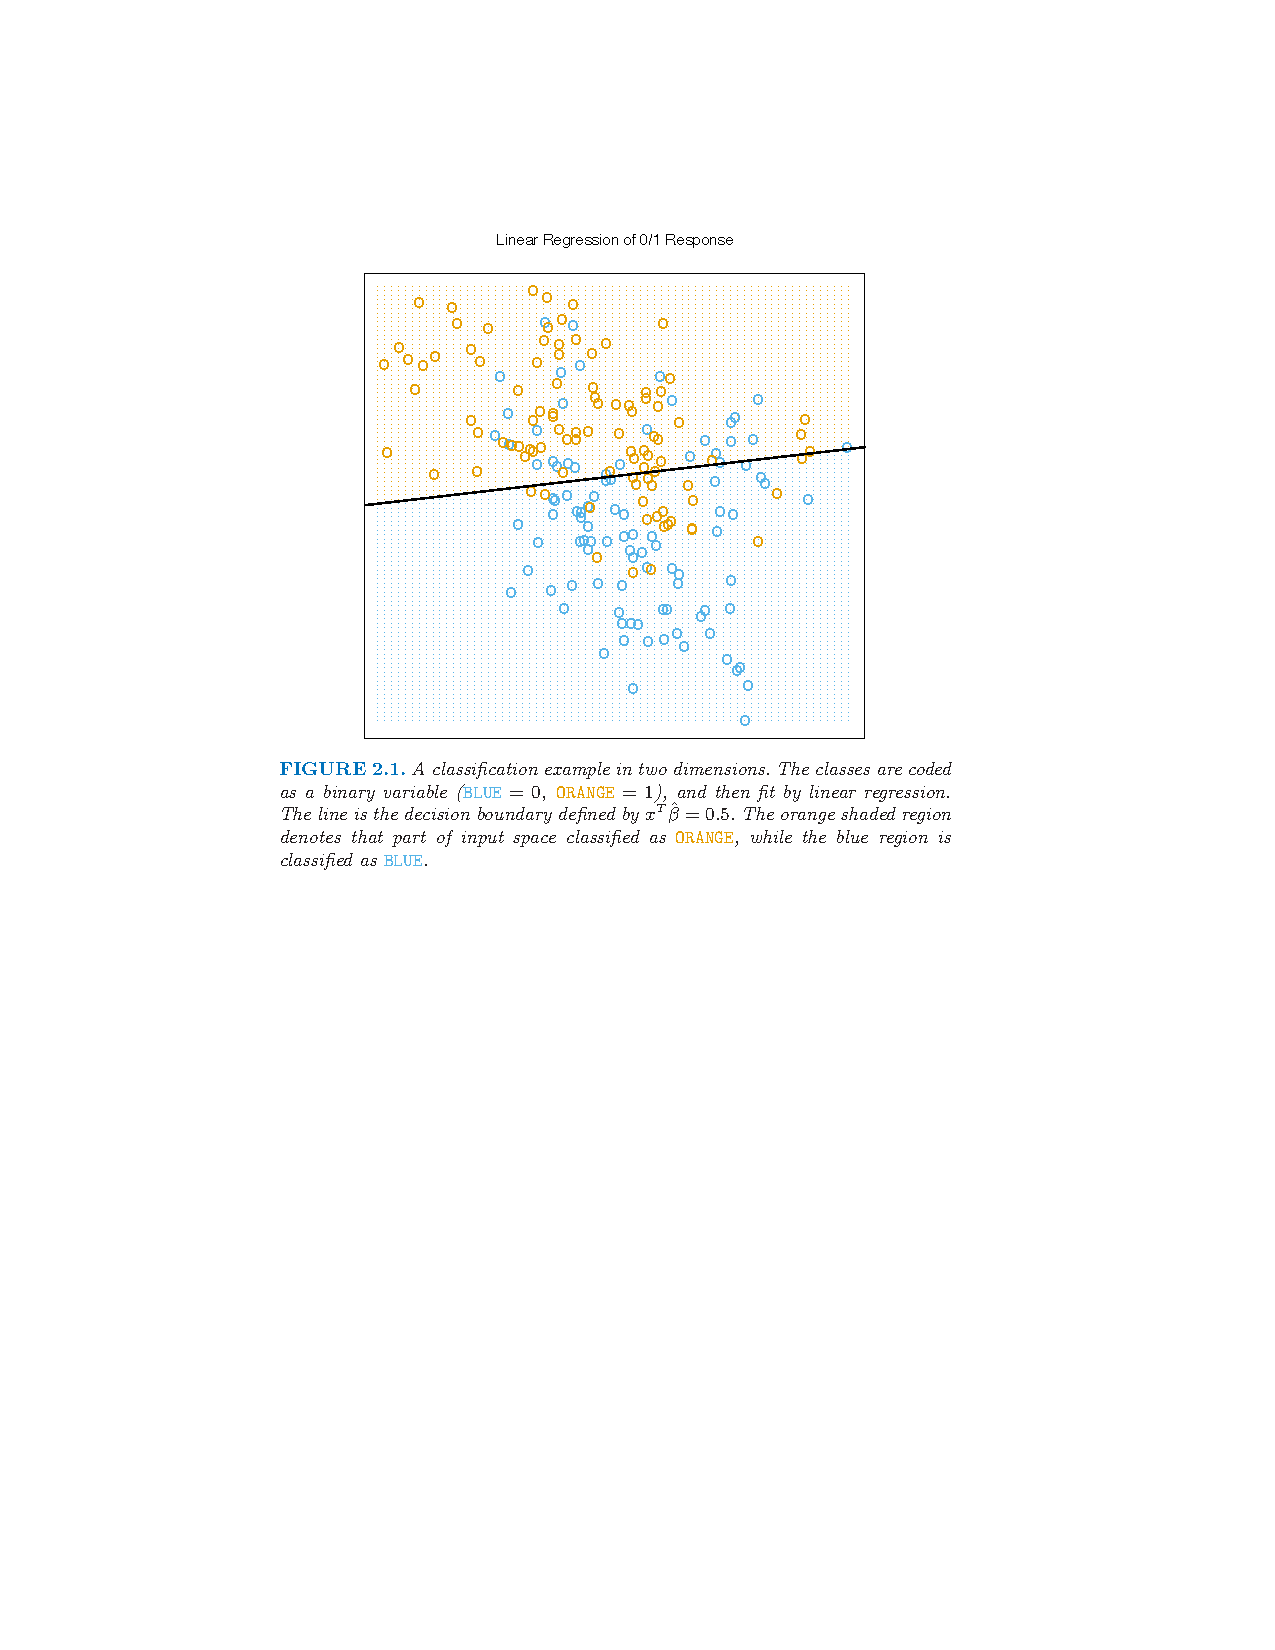
\includegraphics[width=3.5in]{./resources/classifierOLS.pdf}
\label{classOLS}
\end{center}
\end{figure}
\end{frame}


\begin{frame}{Alternative}
\begin{itemize}
\item Lots of potential alternatives to our decision rule.
\item A simple idea is to hold a majority vote of neighboring points 
\begin{eqnarray*}
Y^{*} = \frac{1}{k} \sum_{x_i \in N_k(x)} y_i
\end{eqnarray*}
\item To avoid including ``yourself'' in your neighborhood, we often estimate on one sample and validate on another
\item How many parameters does this model have: None? One? $k$? 
\item Technically it has something like $N/k$.
\item As $N \rightarrow \infty$ this means we have an infinite number of parameters! (This is a defining characteristic of non-parametrics).
\end{itemize}
\end{frame}


\begin{frame}{15 Nearest Neighbor}
\begin{figure}[htbp]
\begin{center}
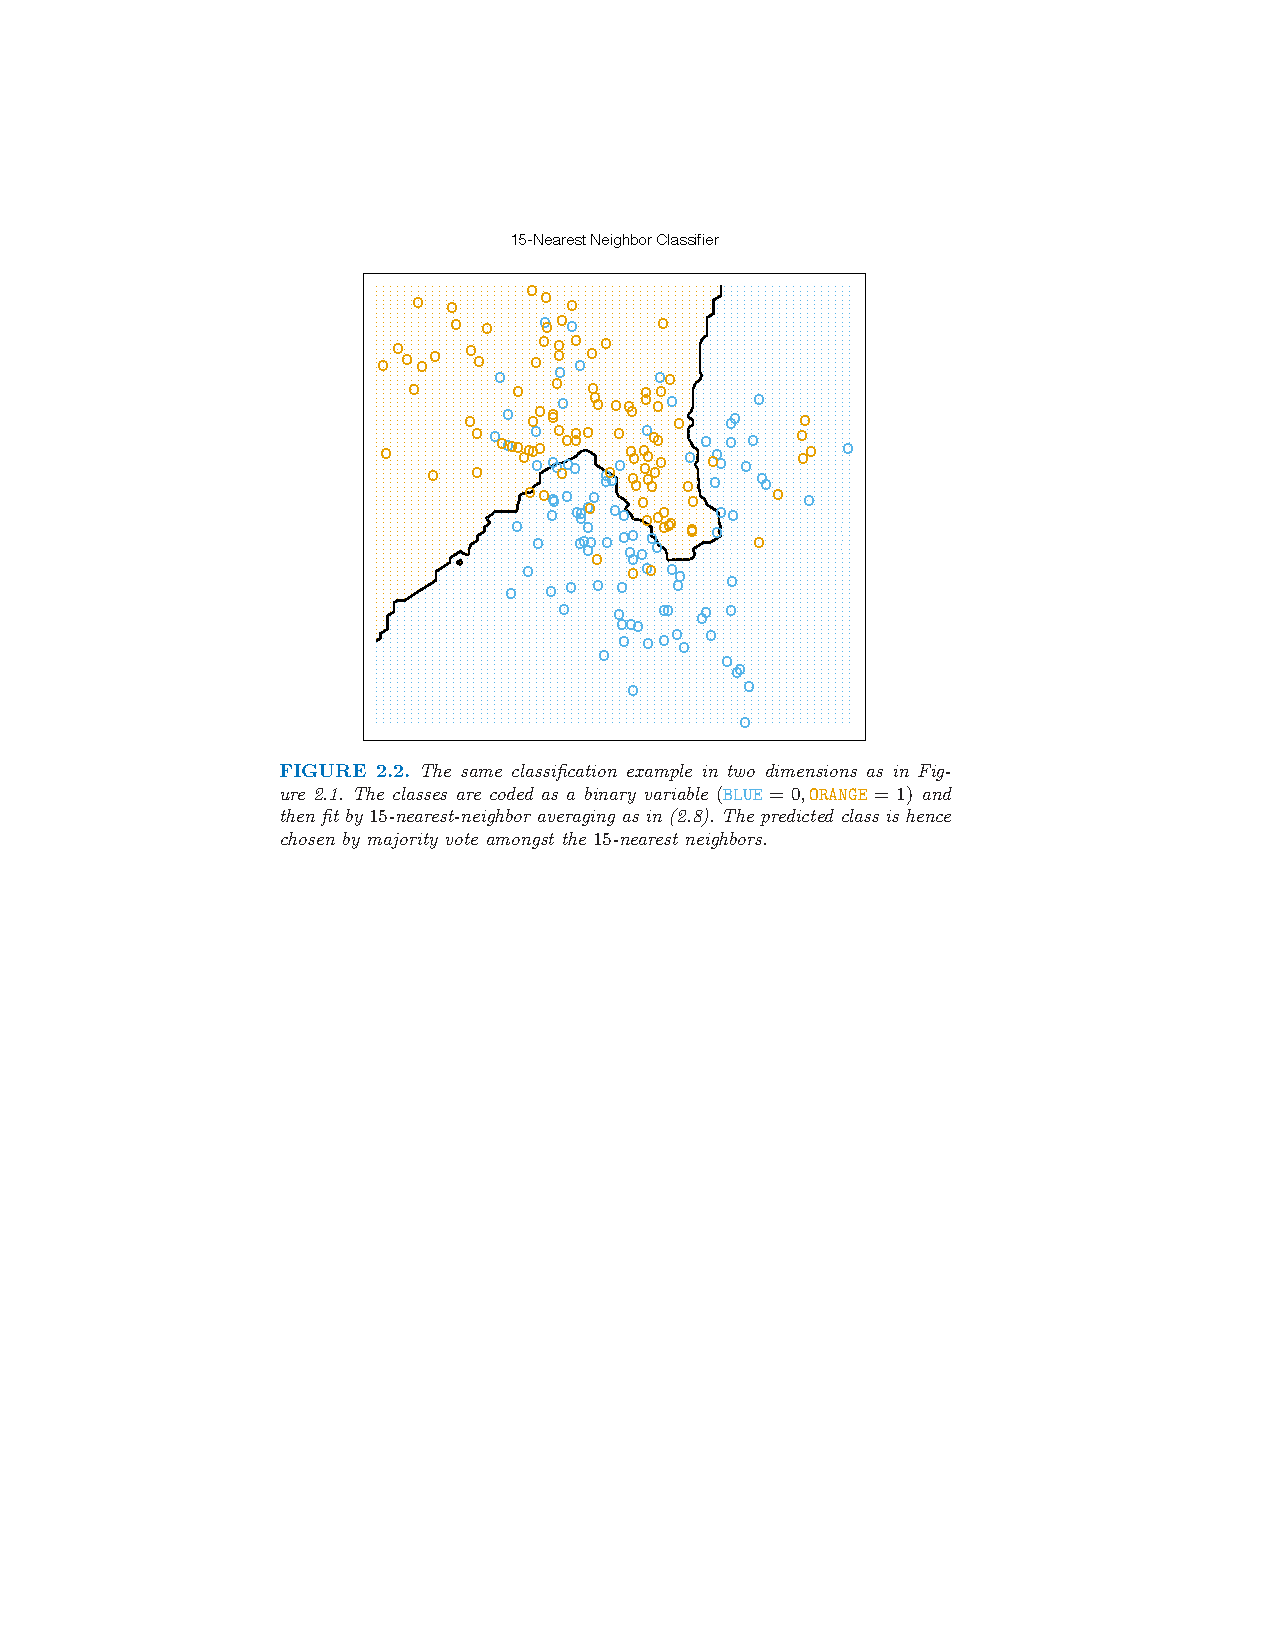
\includegraphics[width=3.5in]{./resources/classifier15nn.pdf}
\label{class15nn}
\end{center}
\end{figure}
\end{frame}

\begin{frame}{Extreme: 1 Nearest Neighbor}
\begin{figure}[htbp]
\begin{center}
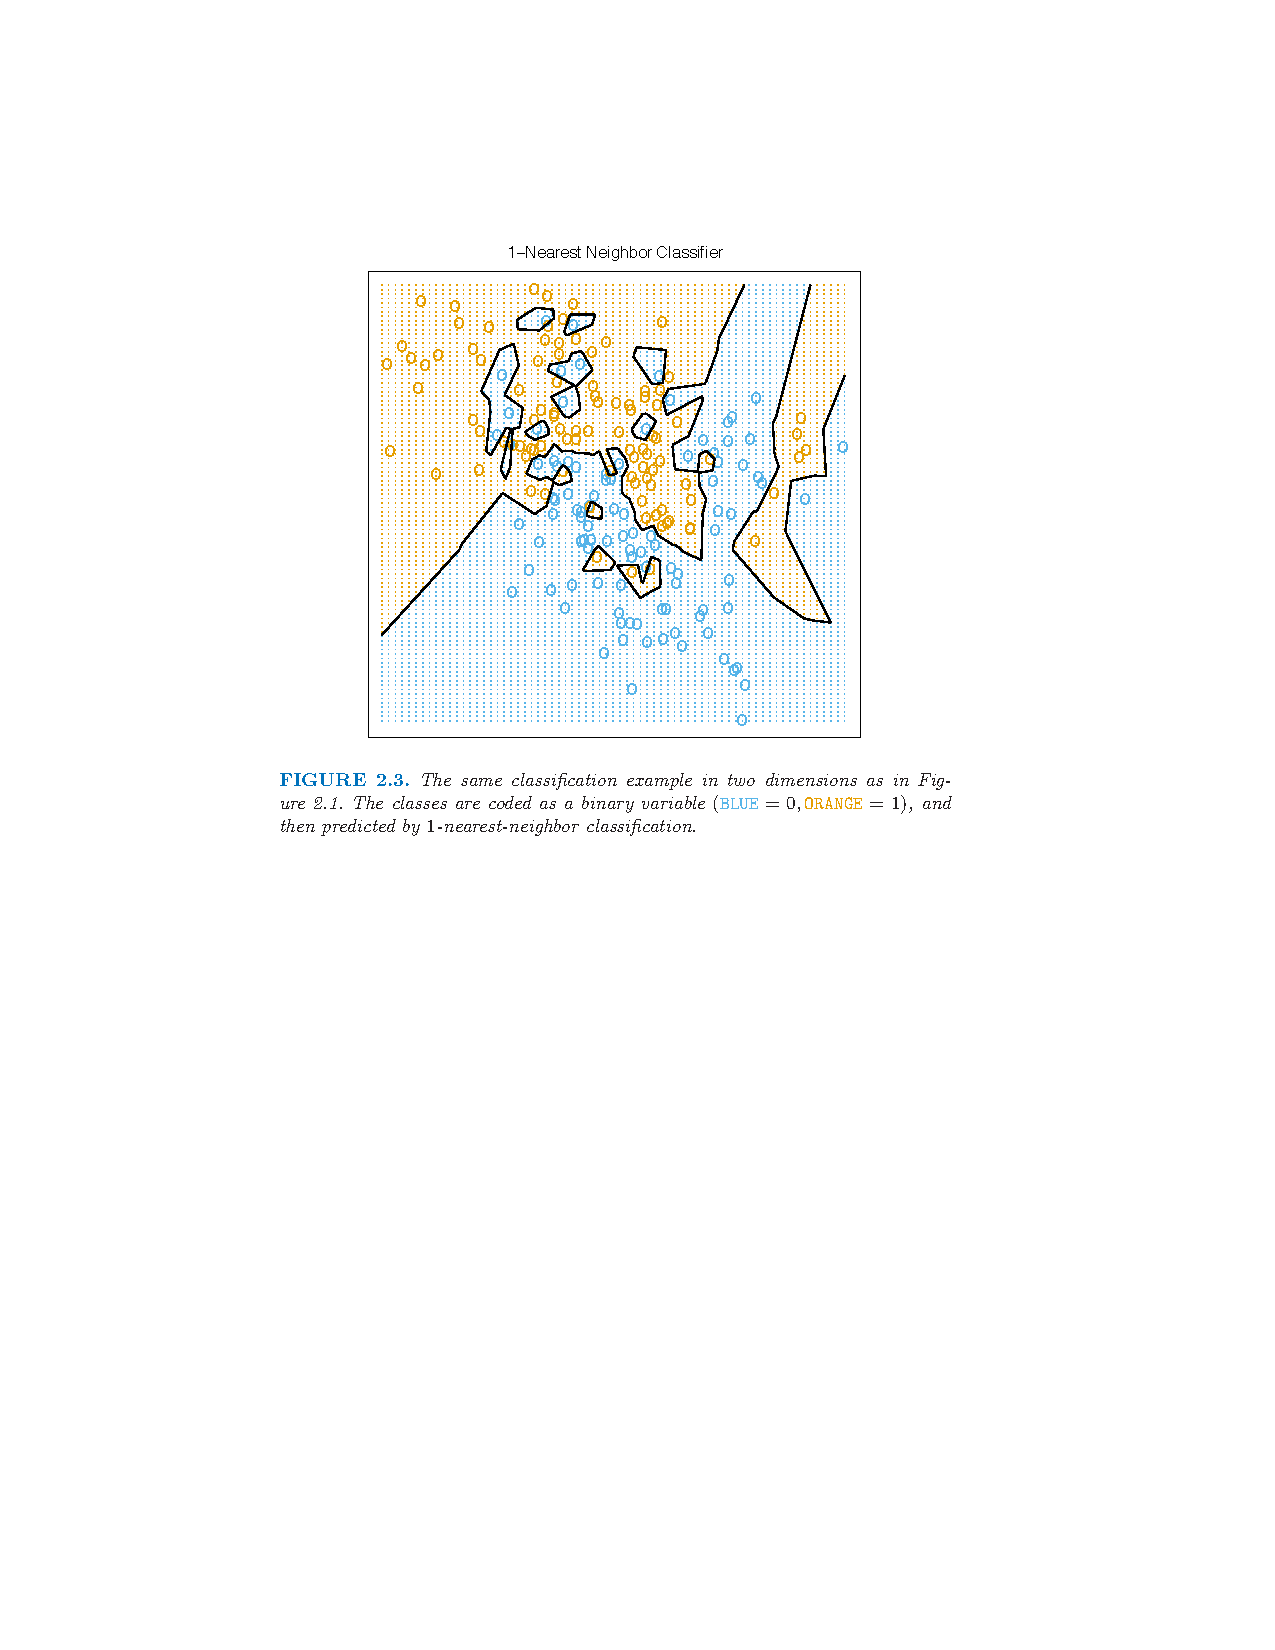
\includegraphics[width=3.5in]{./resources/classifier1nn.pdf}
\label{class15nn}
\end{center}
\end{figure}
\end{frame}

\begin{frame}{Comparisons}
\begin{itemize}
\item What would happen if $K \rightarrow N$?
\item The k-NN model is locally constant.
\item The k-NN approach tends to be really bumpy which can be undesirable.
\item The OLS model is globally linear (is this always true?)
\end{itemize}
\end{frame}
\begin{frame}{What about?}
\begin{itemize}
\item If we fixed the fact that there are discrete jumps in who is in the neighborhood by smoothly weighting observations and varying those weights instead (Kernels).
\item Another drawback of $k-NN$ is that we consider distance in each $X$ dimension on the same scale, perhaps we could rescale the data to improve our ``closeness'' measure.
\item Instead of fitting a constant locally, we fit a linear function locally (Lowess).
\item Instead of using a global linear approximation in OLS use a more flexible nonlinear one.
\item There is a bias/variance tradeoff. \alert{explain}.
\end{itemize}
\end{frame}

\begin{frame}{Bias Variance Decomposition}
We can decompose any estimator into two components
\begin{eqnarray*}
\underbrace{E[(y- \hat{f}(x))^2]}_{MSE} =\underbrace{\left( E[\hat{f}(x) - f(x)] \right)^2}_{Bias^2}  +  \underbrace{E \left[ \left(\hat{f}(x) - E[\hat{f}(x) \right] \right)^2}_{Variance} 
\end{eqnarray*}
\begin{itemize}
\item In general we face a tradeoff between bias and variance.
\item In k-NN as $k$ gets large we reduce the variance (each point has less influence) but we increase the bias since we start incorporating far away and potentially irrelevant information.
\item In OLS we minimize the variance among unbiased estimators assuming that the true $f$ is linear.
\end{itemize}
\end{frame}

\begin{frame}{Bias Variance Decomposition}
What minimizes MSE?
\begin{eqnarray*}
f(x_i) = E[Y_i | X_i] 
\end{eqnarray*}
\begin{itemize}
\item Seems simple enough (but we are back where we started).
\item How do we compute the expectation ?
\item k-NN tries to use local information to estimate conditional mean
\item OLS uses entire dataset and adds structure $ y = x \beta$ to the problem.
\end{itemize}
\end{frame}


\begin{frame}{Big Data}
\begin{itemize}
\item It used to be that if you had $N=50$ observations then you had a lot of data.
\item Those were the days of finite-sample adjusted t-statistics.
\item Now we frequently have 1 million observations or more, why can't we use k-NN type methods everywhere?
\end{itemize}
\end{frame}

\begin{frame}{Curse of Dimensionality}
Take a unit hypercube in dimension $p$ and we put another hypercube within it that captures a fraction of the observations $r$ within the cube
\begin{itemize}
\item Since it corresponds to a fraction of the unit volume, $r$ each edge  will be $e_p(r) = r^{1/p}$.
\item $e_{10}(0.01) = 0.63$ and $e_{10}(0.1) = 0.80$, so we need almost 80\% of the data to cover 10\% of the sample!
\item If we choose a smaller $r$ (include less in our average) we increase variance quite a bit without really reducing the required interval length substantially.
\end{itemize}
\end{frame}

\begin{frame}{Curse of Dimensionality}
\begin{figure}[htbp]
\begin{center}
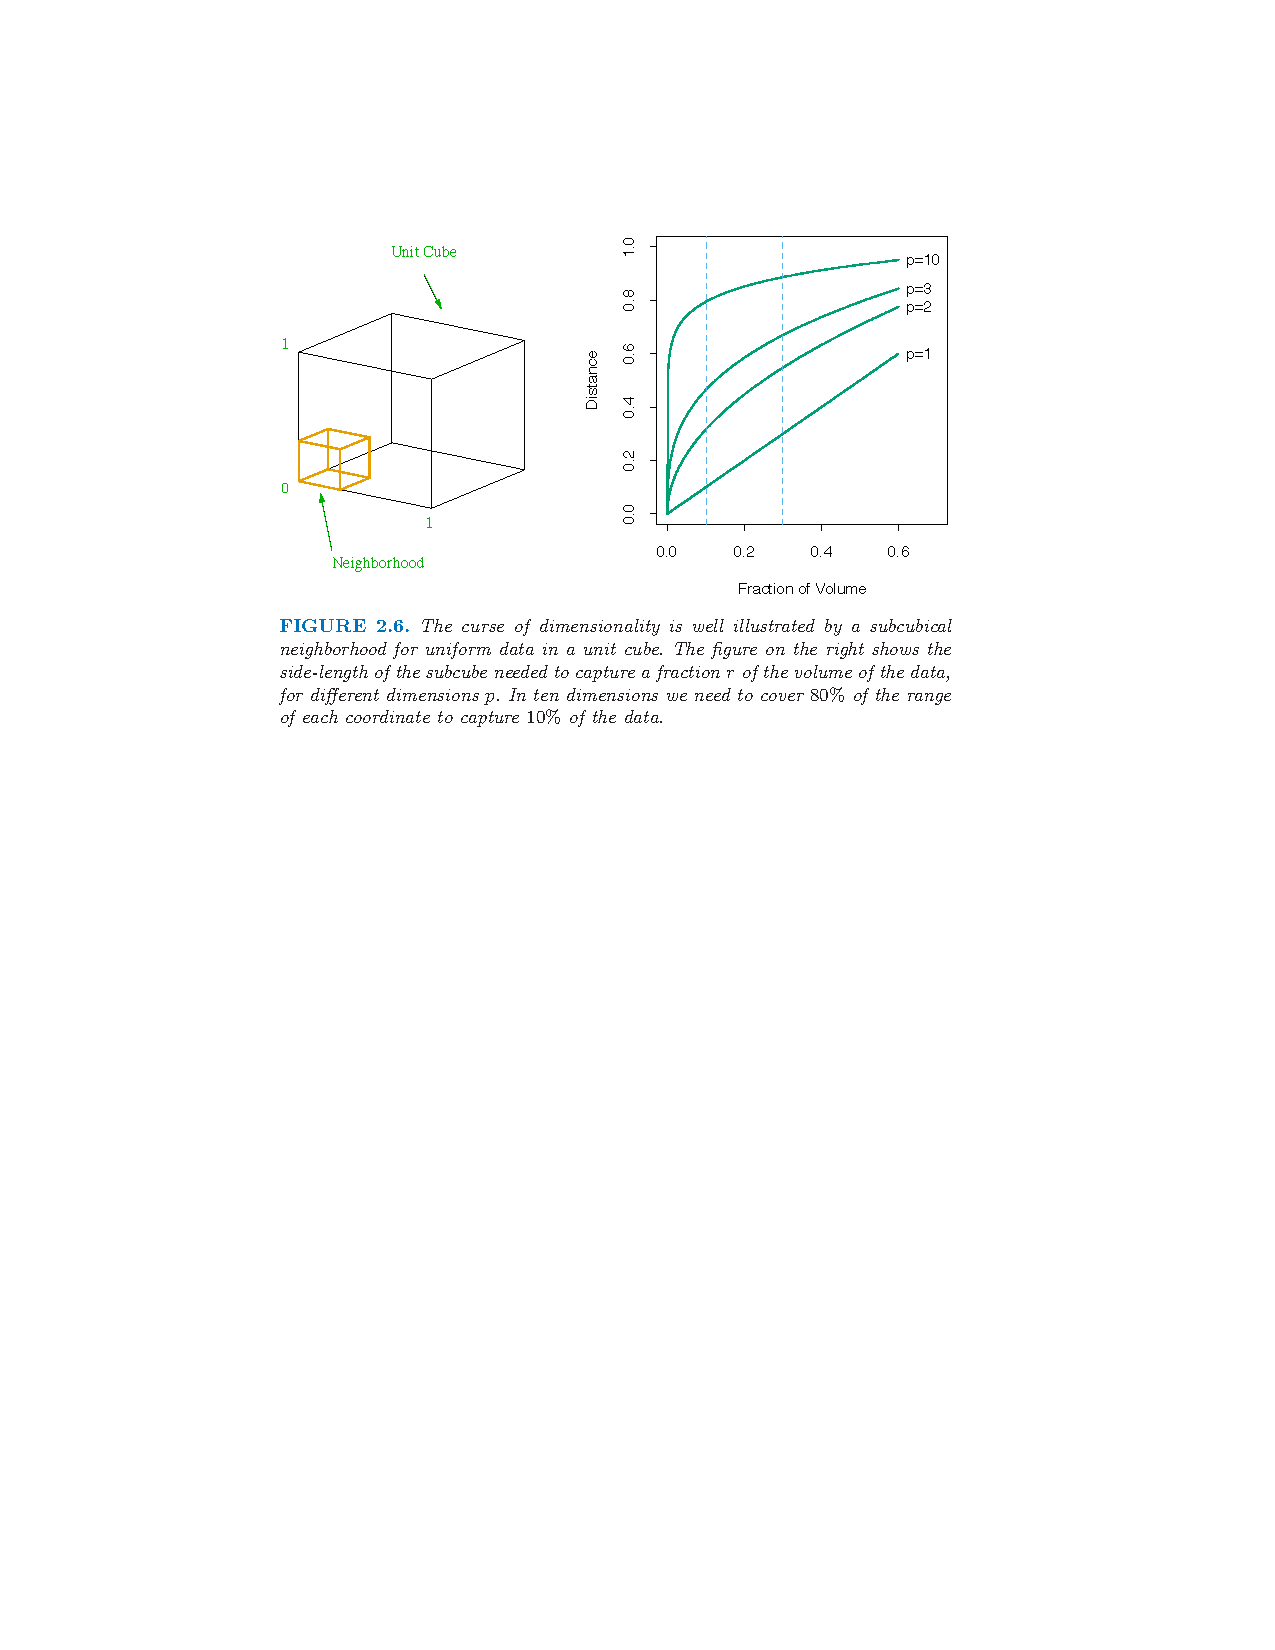
\includegraphics[width=3.5in]{./resources/figure26.pdf}
\label{class15nn}
\end{center}
\end{figure}
\end{frame}

\begin{frame}{Curse of Dimensionality}
Don't worry, it only gets worse:
\begin{eqnarray*}
d(p,N) = \left(1-\left(\frac{1}{2} \right)^{1/N} \right)^{1/p}
\end{eqnarray*}

\begin{itemize}
\item $d(p,N)$ is the distance from the origin to the closest point.
\item $N=500$ and $p=10$ means $d = 0.52$ or that the closest point is closer to the boundary than the origin!
\item Why is this a problem?
\item In some dimension nearly every point is the closest point to the boundary -- when we average over nearest neighbors we are \alert{extrapolating} not \alert{interpolating}.
\end{itemize}
\end{frame}


\begin{frame}{Density/Distribution Estimation}
One of the more successful and popular uses of nonparametric methods is estimating the density or distribution function $f(x)$ or $F(x)$.
\begin{itemize}
\item Estimating the CDF is easy and something you have already done
\item Q-Q plots, etc.
\end{itemize}
\begin{eqnarray*}
\hat{F}_{ECDF}(x_0) = \frac{1}{N} \sum_{i=1}^N (x_i \leq x_0 )
\end{eqnarray*}
\begin{itemize}
\item Differentiating to get density is unhelpful : $F_{ECDF}'(x) = 0$ in most places.
\end{itemize}
\end{frame}

\begin{frame}{Density/Distribution Estimation}
One of the more successful and popular uses of nonparametric methods is estimating the density or distribution function $f(x)$ or $F(x)$.
\begin{itemize}
\item Think about the histogram (definition of derivative):
\begin{eqnarray*}
\hat{f}_{HIST}(x_0) = \frac{1}{N} \sum_{i=1}^N \frac{\mathbf{1}(x_0 - h < x_i < x_0 + h)}{2 h}
\end{eqnarray*}
\end{itemize}
\end{frame}

\begin{frame}{Density/Distribution Estimation}
\begin{itemize}
\item Divide the dataset into bins, count up fraction of observations in each bins
\item Similar to k-NN except instead of windows that vary with $x_i$ we have fixed width bins
\item Larger bin width $\rightarrow$ More Bias, Less Variance.
\item Histogram will never be smooth! (Just like k-NN).
\end{itemize}
\begin{eqnarray*}
\hat{f}_{HIST}(x_0) = \frac{1}{Nh} \sum_{i=1}^N  \frac{1}{2} \cdot \mathbf{1} \left (\left|\frac{x_i - x_0}{h} \right| < 1 \right)
\end{eqnarray*}
\end{frame}




\begin{frame}{Smooth Kernels}
We can take our histogram and smooth it out:
\begin{eqnarray*}
\hat{f}(x_0) = \frac{1}{Nh} \sum_{i=1}^N  K  \left(\frac{x_i - x_0}{h} \right)  \frac{1}{n}\sum_{i=1}^n K_h\left(
y-y_i\right).
\end{eqnarray*}
We call $K(\cdot)$ a \alert{Kernel function} and $h$ the \alert{bandwidth}. We usually assume
\begin{enumerate}[(i)]
\item $K(z)$ is symmetric about $0$ and continuous.
\item $\int K(z) d z = 1$,  $\int z K(z) d z = 0$,  $\int |K(z)| d z < \infty$.
\item Either (a) $K(z) = 0$ if $|z| \geq z_0$ for some $z_0$ or \\
(b) $|z| K(z) \rightarrow 0$ as $|z| \rightarrow \infty$.
\item $\int z^ K(z) d z = \kappa$ where $\kappa$ is a constant.
\end{enumerate}
\end{frame}

\begin{frame}{Kernel Smoothers}
If $K$ is $C^k$, then so is ${\hat f}_n$, so we can plot it nicely.

\pause

Usually we choose a smooth, symmetric $K$:



\pause




\begin{itemize}[<+->]
\item $K=\phi$, density of $N(0,1)$ (or some other symmetric density);
\item $K$ with compact support: Epanechnikov (mildly) optimal
\[
K(x)= \frac{3}{4} \max(1-x^2,0).
\]
\end{itemize}
\pause
A common nonsmooth choice: $K(x)=(|x|<1/2)$ gives the {\em histogram}
estimate.
\end{frame}

\begin{frame}{Kernel Comparison}
\begin{figure}[htbp]
\begin{center}
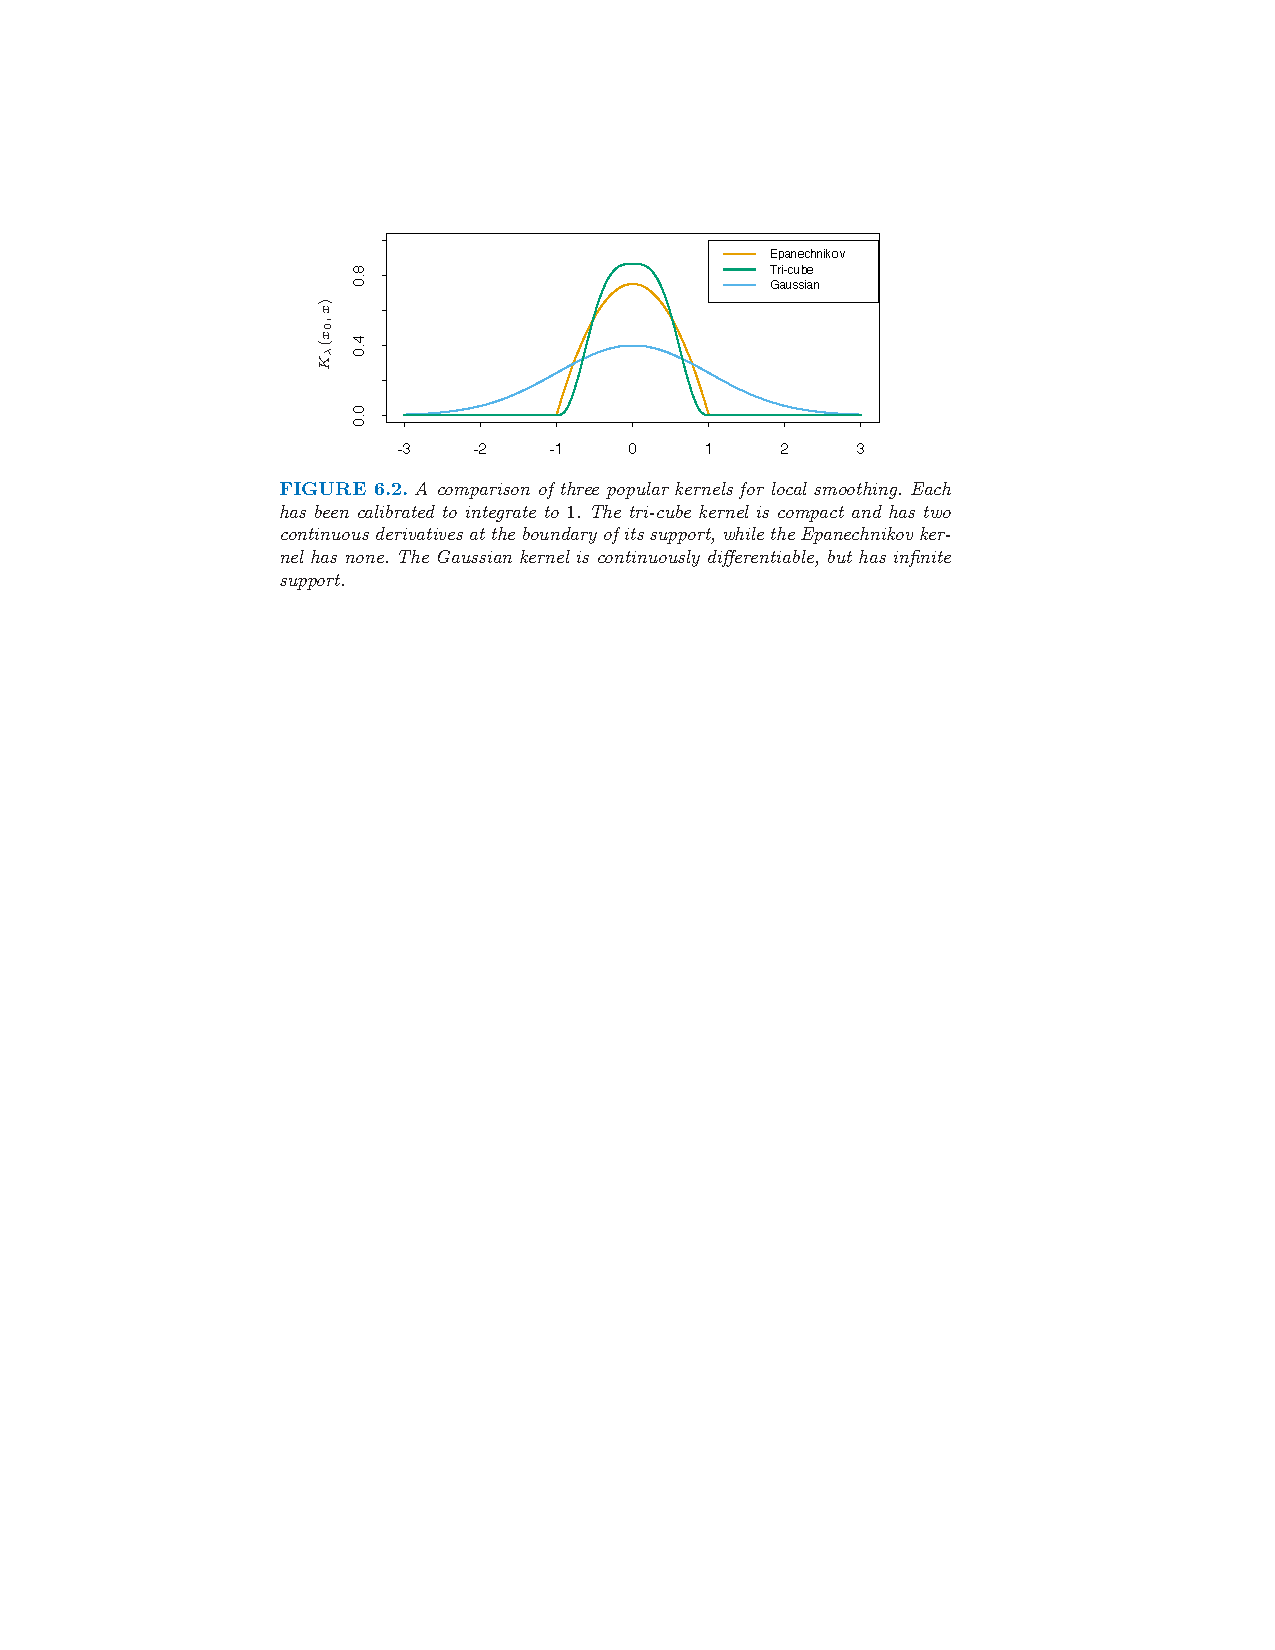
\includegraphics[width=3.5in]{./resources/kernelfig.pdf}
\label{classOLS}
\end{center}
\end{figure}
\end{frame}


\begin{frame}{How to Choose $h$}
\begin{itemize}
\item We want both bias and variance to be as small as possible, as usual. 
\item In parametric estimation, it is not a problem: they both go to zero as sample size increases.
\end{itemize}
 {\bf Problem with nonparametrics:}
$$E\hat{f}_n(y)=\int K((y-t)/h)f(t)dt/h=\int K(-u)f(y+uh)du=f(y)+O(h^2)$$
$\rightarrow$ bias can be made tiny by having a very concentrated kernel ($h\simeq 0$);
but 
$$V\hat{f}_n(y)=\frac{1}{nh^2}VK((y-Y)/h)=O\left(\frac{1}{nh}\right)$$
$\rightarrow$ a small $h$ gives a high variance! \\
Reducing $h$ reduces bias, but increases variance; how are we to
trade off?
\end{frame}

\begin{frame}{The AMISE}
\begin{itemize}
\item  Asymptotic Mean Integrated Square Error =asymptotic approximation of a quadratic loss function
$$E\left({\hat f}_n(y)-f(y)\right)^2 dy$$
\item Simple approximate expression (symmetric kernels of order 2): $$(\mbox{bias})^2+\mbox{variance}= A
h^4+B/nh$$
\item {\bf Why?} Bias in $y$ is
$$
\int K(-u)\left(f(y+uh)-f(y)\right)du \simeq h^2 \frac{f''(y)}{2}\int K(u)u^2 du.
$$
{\em Intuition:} if $f$ is close to linear around $y$, then averaging
does not hurt us: $f"(y)\simeq 0$ and the bias is small. The bias is larger  (and negative) at the mode of $f$.
\end{itemize}
\end{frame}

\frame{\frametitle{The Variance}

\pause

\[
V\hat{f}_n(y)=\frac{1}{nh^2} VK((y-Y)/h)
\]

\pause

The important term in 
\[
VK((y-Y)/h)
\]
is 
\[
h\int K(u)^2 f(y+uh)du\simeq h f(y)\int K(u)^2 du.
\]

\pause

And we end up with 
\[
V\hat{f}_n(y) \simeq \frac{f(y)}{nh} \int K(u)^2du.
\]

\pause

{\em Intuition:} we are really taking an average over $nhf(y)$
points. In low-density region, this induces a high \emph{relative\/}
imprecision:
\[
\frac{\sigma(\hat{f}_n(y))}{f(y)}=\frac{1}{nhf(y)} \int K(u)^2du.
\]
 }

\frame{\frametitle{Optimal bandwidth}
\begin{itemize}
\item The AMISE is $$Ah^4+B/nh$$
 with $A=\int \left(f''(y)\right)^2 \left(\int u^2K\right)^2 /4$ and $B=f(y)\int K^2$
\item  AMISE is
smallest in $h^*_n=\left(\frac{B}{4An}\right)^{1/5}$. Then,
\begin{itemize}[<+->]
\item bias and standard error are \emph{both} in $n^{-2/5}$
\item and the AMISE is $n^{-4/5}$---{\bf not} $1/n$ as it is in parametric models.
\end{itemize}
\item But: $A$ and $B$ both depend on $K$ (known) and $f(y)$ (unknown), and
especially ``wiggliness''
$\int (f'')^2$ (unknown, not easily estimated). Where do we go from here? 
\end{itemize}
}


\frame{\frametitle{Silverman's Rule of Thumb}
\begin{itemize}
\item If $f$ is normal with variance $\sigma^2$ (may not be a very appropriate benchmark!), the optimal bandwidth
is
$$h^*_n=1.06 \sigma n^{-1/5}$$
\item Just do it with $\sigma=s$ empirical dispersion of the $y_i$'s , or
something more robust/slightly less smooth:
$$h^*_n=0.9*\min(s,IQ/1.34)*n^{-1/5}, \; \mbox{IQ=interquartile
 distance}$$
\item Investigate changing it by a reasonable multiple.
\end{itemize}
}

\frame{\frametitle{Cross-validation}
\begin{itemize}
\item General concept in the whole of nonparametrics: choose $h$ to minimize
a criterion $CV(h)$ that approximates
$$ AMISE(h)=\int E(\hat{f}_n(x)-f(x))^2dx.$$
\item Usually programmed in metrics software. \emph{If you can do it, do it on a subsample, and rescale.}
\item Two problems:

\begin{itemize}[<+->]
\item it is costly; often it involves computing ``leave-one-out''
  estimators
\[
\hat{f}_{(-i)}(x_i)=\frac{1}{nh}\sum_{j\neq i}
K\left(\frac{x_i-x_j}{h}\right),
\]
for {\em every\/} observation $i$.
\item the resulting $h$ converges super-slowly ($n^{-1/10}$!) to the
  optimal one. 
\end{itemize}
\end{itemize}
}

\begin{frame}{Alternatives to Cross-Validation}
\begin{itemize}
\item LOOCV
\item k-fold CV
\item Sample Splitting
\begin{itemize}
\item Training Set
\item Test Set
\item Validation Set
\end{itemize}
\end{itemize}
\end{frame}



\frame{\frametitle{Local Bandwidths}

\pause

If you only care about $f(y)$ at some given point, then 
\[
A=f''(y)^2 \left(\int u^2K\right)^2/4 \mbox{ and } B=f(y)\int K^2.
\]

\pause

So in a low-density region, worry about variance and take $h$ larger.
In a curvy region, worry about bias and take $h$ small.
 
}

\frame{\frametitle{Higher-Order Kernels}
\begin{itemize}
\item $K$ of order $r$ iff $\int x^j K(x) dx=0$ for $j<r$ and $\int x^r
K(x)dx \neq 0$. Try $r>2$?
\item The beauty of it: bias in $h^r$ if $f$ is at least $C^r$\ldots so AMISE can be
reduced to $n^{-r/(2r+1)}$, almost $\sqrt{n}$-consistent if $r$ is
large. 
\item But gives wiggly (and sometimes negative) estimates
$\rightarrow$ leave them to theorists. 
\end{itemize}
}

\begin{frame}{Back to the CDF}
\small
Since now we have estimated the density with
\begin{align*}
{\hat f}_n(y)= \frac{1}{nh}\sum_{i=1}^n K\left(
\frac{y-y_i}{h}\right),
\end{align*}
a natural idea is to integrate; let $\mathcal{K}(y)=\int_{-\infty}^y K(t)dt$, try
\begin{align*}
{\hat F}_n(y)= \frac{1}{n}\sum_{i=1}^n \mathcal{K}\left(
\frac{y-y_i}{h}\right)
\end{align*}
as a reasonable estimator of the cdf in $y$.
Very reasonable indeed:
\begin{itemize}
  \item when $n \longrightarrow \infty$ and $h$ goes to zero (at rate
    $n^{-1/3}$\ldots) 
it is consistent at rate $\sqrt{n}$
\item it is nicely smooth and accords well with the density estimator
\item \ldots\ it is a much better choice than the empirical cdf.
\end{itemize}
\end{frame}


\frame{\frametitle{What if $y$ is of dimension $p_y>1$?}

\pause

``Easy'': use $p_y$-dimensional $K$ (often a $p_y$-product of 1-dim
kernels) and bandwidth $h$, and do

\pause


\[
{\hat f}_n(y)= \frac{1}{nh^p_y}\sum_{i=1}^n K\left(
\frac{y-y_i}{h}\right).
\]

\begin{itemize}
\item {\bf 1st minor pitfall:} the various dimensions may have very
different variances, so use  $(h_1,\ldots,h_{p_y})$.
\item {\bf 2nd minor pitfall:} they may be strongly correlated; then
sphericize first.
\item {\bf Major problem:} next slide\ldots
\end{itemize}
 }

 \frame{\frametitle{The Curse of Dimensionality}

\pause

\begin{itemize}
\item Computational cost increases exponentially.
\item {\em Much worse:} to achieve precision $\epsilon$ in dimension $p_y$, the number of
  observations you need increases as
\[
n \simeq \epsilon^{-(2+p_y/2)}.
\]
\item The {\em empty space\/} phenomenon: 
if $(y_1,\ldots,y_{p_y})$ all are iid uniform on $[-1,1]$, then only
$n/(10^{p_y})$ observations on average have all components in
$[-0.1,0.1]$. Bias still in $h^2$, but variance in $1/nh^{p_y}$ now.
\end{itemize}
}

\frame{\frametitle{Silverman's Table}

\pause

 Silverman (1986 book) 
provides a table illustrating the difficulty of kernel estimation
in high dimensions. To estimate the density at 0 of a $N(0,1)$ with
a given accuracy, he reports:

\pause

\begin{table}
\begin{center}
\vspace{1ex}
\begin{tabular}{|c|c|}\hline
Dimensionality Required & Sample Size    \\
\hline
1               &  4    \\
2               &  19    \\
5           & 786 \\
7          & 10,700 \\
10           & 842,000 \\
\hline
\end{tabular}
\end{center}
\end{table}

\pause

{\bf Not to be taken lightly\ldots} in any case convergence  with
the optimal bandwidth  is in $n^{-2/(4+p_y)}$ now---and Silverman's
rule of thumb for choosing $h^*_n$ must be adapted too. }

\frame{\frametitle{Usually we care about conditional densities}

\pause

That is: we have covariates $x$, we want the density $f(y|x)$. Again, ``easy'':

\pause

\begin{enumerate}
\item get a kernel estimator of the joint density $f(y,x)$;
\item and one of of the marginal density $f(x)$;
\item then define
\[
\hat{f}_n(y|x)=\frac{\hat{f}_n(y,x)}{\hat{f}_n(x)}=\frac{\frac{1}{n
h_y^{p_y}h_x^{p_x}}\sum_{i=1}^n
K\left(\frac{y-y_i}{h_y}\right)K\left(\frac{x-x_i}{h_x}\right)}{\frac{1}{h_y^{p_y}}
\sum_{i=1}^n K\left(\frac{x-x_i}{h_x}\right)}.
\]
\end{enumerate}

\pause

But the joint density is $(p_x+p_y)$ dimensional\ldots\ and the curse
strikes big time.

}




\frame{\frametitle{What if my distribution is discrete-continuous?}
Very often in microeconometrics some covariates only take discrete
values (e.g. gender, race, income bracket\ldots). Say the only discrete variable is gender, we care about the density of income of men. 
\begin{itemize}
\item The kernel approach adapts directly: we separately
estimate a density for men (on the corresponding subsample).
\item {\em Better:}  mix the two subsamples! Add women, but  {\bf with a small weight $w$}.
\item Intuition: by doing so we increase the bias (the density for women is
probably different than for men) $\rightarrow$  bad, in $w^2$ but we reduce the variance, by $O(w)$; and this dominates for small $w$. (cf Li-Racine).
\end{itemize}
}

 \frame{\frametitle{The
Seminonparametric Approach}
\begin{itemize}
\item If we are ``pretty sure'' that $f$ is almost $f_{m,\sigma}$ for some
family of densities indexed by  $(m,\sigma)$, then we can choose a family of positive functions of increasing complexity  $P^1_\theta,P^2_\theta,\ldots$
\item Choose some $M$ that goes to infinity as $n$ does (more slowly), and
maximize over $(m,\sigma,\theta)$ the loglikelihood

\[
\sum_{i=1}^n \log f_{m,\sigma}(y_i)P^M_\theta(y_i).
\]
It works\ldots but it is hard to constrain it to be a density for
large $M$. \end{itemize}}



\frame{\frametitle{Mixtures of Normals}

\pause

A special case of seminonparametrics, and
usually a very good approach: Let $y|x$ be drawn from

\pause

\begin{description}
\item[] $N(m_1(x,\theta),\sigma^2_1(x,\theta))$ with probability
$q_1(x,\theta)$;
\item[] \ldots
\item[] $N(m_K(x,\theta),\sigma^2_K(x,\theta))$ with probability
$q_K(x,\theta).$
\end{description}
where you choose some parameterizations, and the $q_k$'s are positive
and sum to 1.

\pause

Can be estimated by maximum-likelihood:


\[
\max_{\theta} \sum_{i=1}^n  \log\left(
\sum_{k=1}^K
\frac{q_k(x_i,\theta)}{\sigma_k(x,\theta)}
\phi\left(\frac{y_i-m_k(x_i,\theta)}{\sigma_k(x_i,\theta)}\right)\right).
\]


\pause

Usually works very well with $K\leq 3$ (perhaps after transforming
$y$ to $\log y$, e.g).


}


\frame{\frametitle{Nonparametric Regression}

\pause

Data $(y_i,x_i)_{i=1}^n$ now, we are after $E(g(y,x)|x)=m(x)$ for
some function $g$.
\begin{itemize}
\item Best-fit approach, quite unbiased:
\begin{itemize}[<+->]
\item
if $x=x_i$ then ${\hat m}_n(x)=g(y_i,x_i)$; otherwise \ldots whatever.
\end{itemize}
 But: very jagged estimate; variance independent of $n$, so not
consistent.
\item Better and most usual: Nadaraya-Watson, inspired from kernel idea:
\[
{\hat m}_n(x)=\frac{\sum_{i=1}^n g(y_i,x_i)
K\left(\frac{x-x_i}{h}\right)}{\sum_{i=1}^n
K\left(\frac{x-x_i}{h}\right)}.
\]
again, bias in $h^2$ and variance in $1/nh$ if $p_x=1$.

\pause

{\em Pitfall 1:} very unreliable where  $f(x)$ is small.

\pause

{\em Pitfall 2:} the formal for the optimal bandwidth $h$  is very ugly.
\end{itemize}
}

\frame{\frametitle{Choosing $h$}
\begin{itemize}
\item Plug-in estimates work badly.
\item Fortunately, cross-validation amounts to
\[
\min_h \sum_{i=1}^n
\frac{\left(g(y_i,x_i)-\hat{m}_n(x_i;h)\right)^2}{1-k_i(h)}
\]
where $k_i(h)=K_h(0)/\sum_{j=1}^n K_h(x_i-x_j).$ 
\item So not that hard, and can be done on a subsample and rescaled.
\end{itemize}
}

\frame{\frametitle{Local Linear Regression}
\begin{itemize}
\item The Nadaraya-Watson  estimator in $x$ can be obtained very simply by regressing $g(y_i,x_i)$ on 1, weighting each
observation by $K((x-x_i)/h)$.
\item We could also regress on 1 and  $(x-x_i)$ (going to  higher terms
has problems) instead;\\
Advantages:
\begin{itemize}
\item the bias becomes 0 if the true $m(x)$ is linear.
\item the coefficient of $(x-x_i)$ estimates $m'(x)$.
\item behaves better in ``almost empty'' regions.
\end{itemize}
{Disadvantages:} hardly any, just do it!
\end{itemize}

 }
 
 \begin{frame}{Local Linear}
\begin{figure}[htbp]
\begin{center}
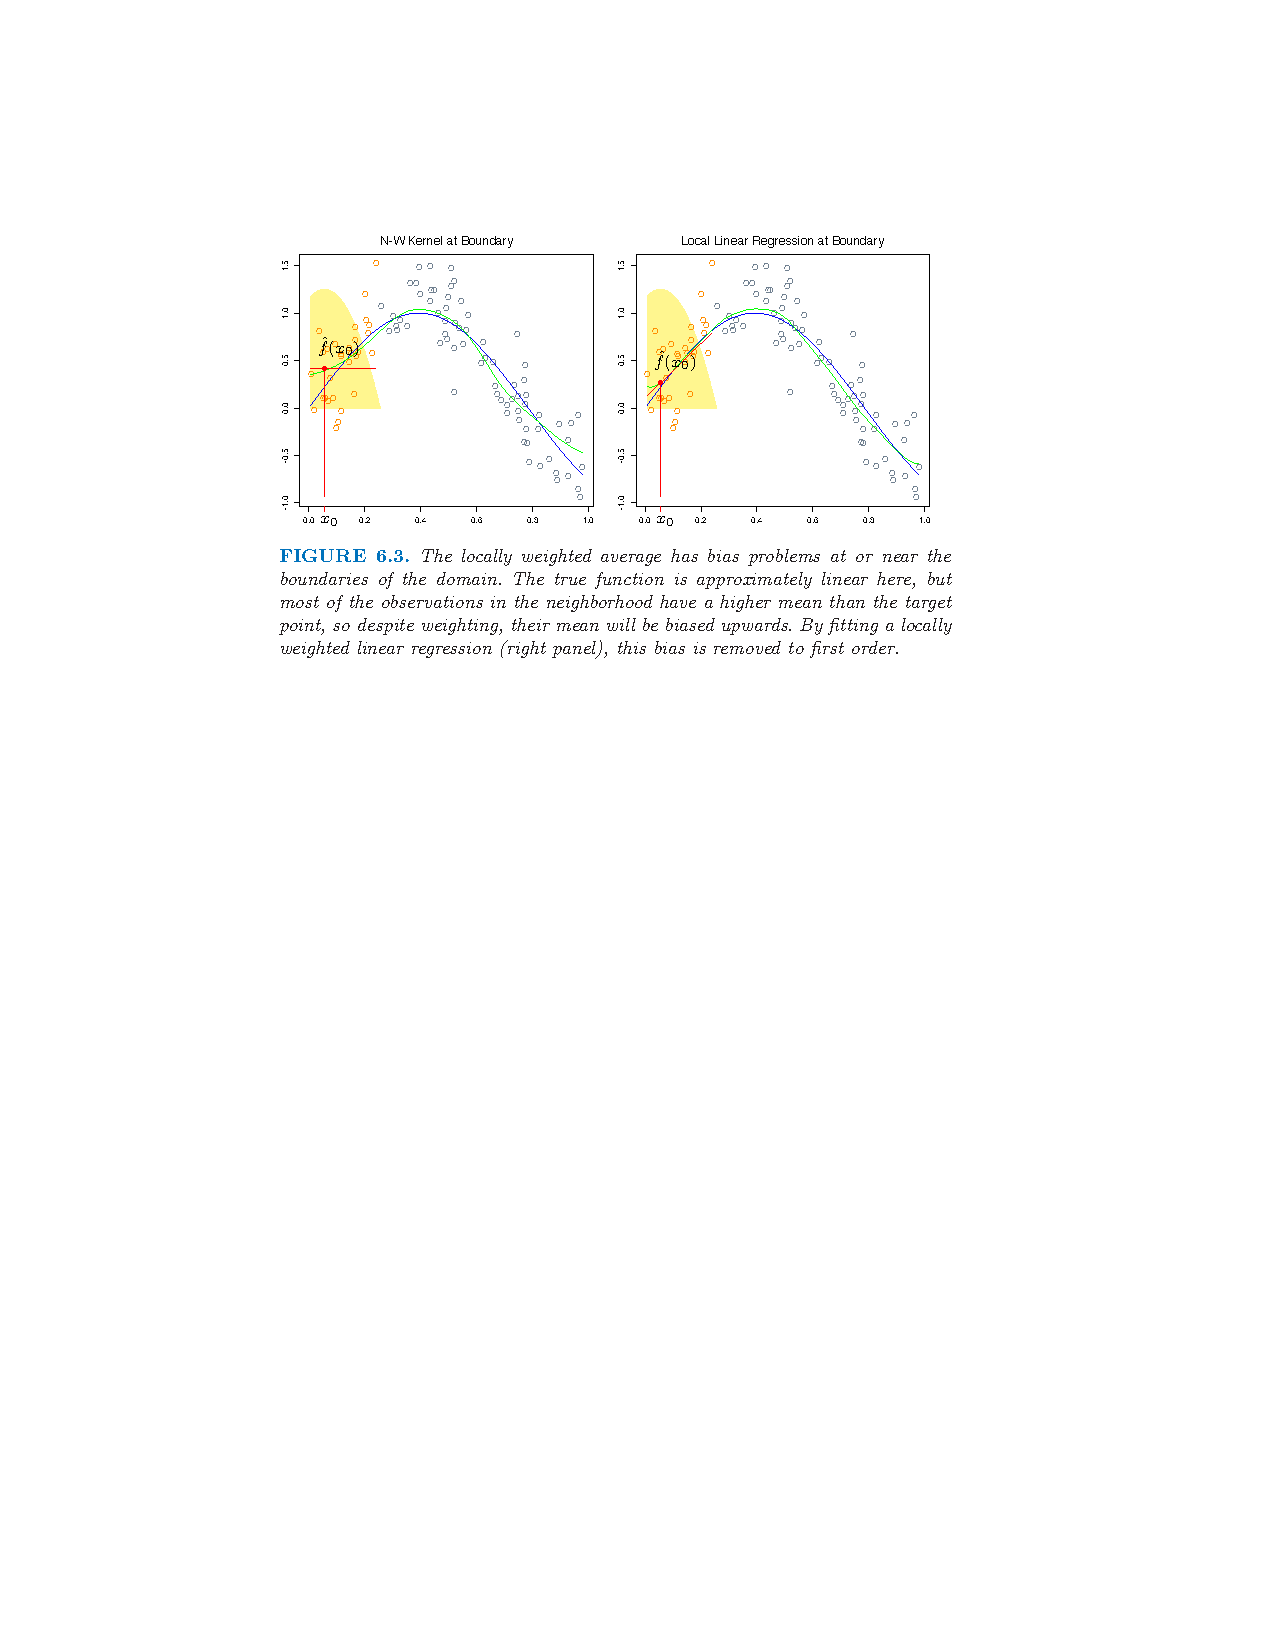
\includegraphics[width=3.5in]{./resources/nwloclinear.pdf}
\label{loclinear1}
\end{center}
\end{figure}
\end{frame}

 \begin{frame}{Local Linear}
\begin{figure}[htbp]
\begin{center}
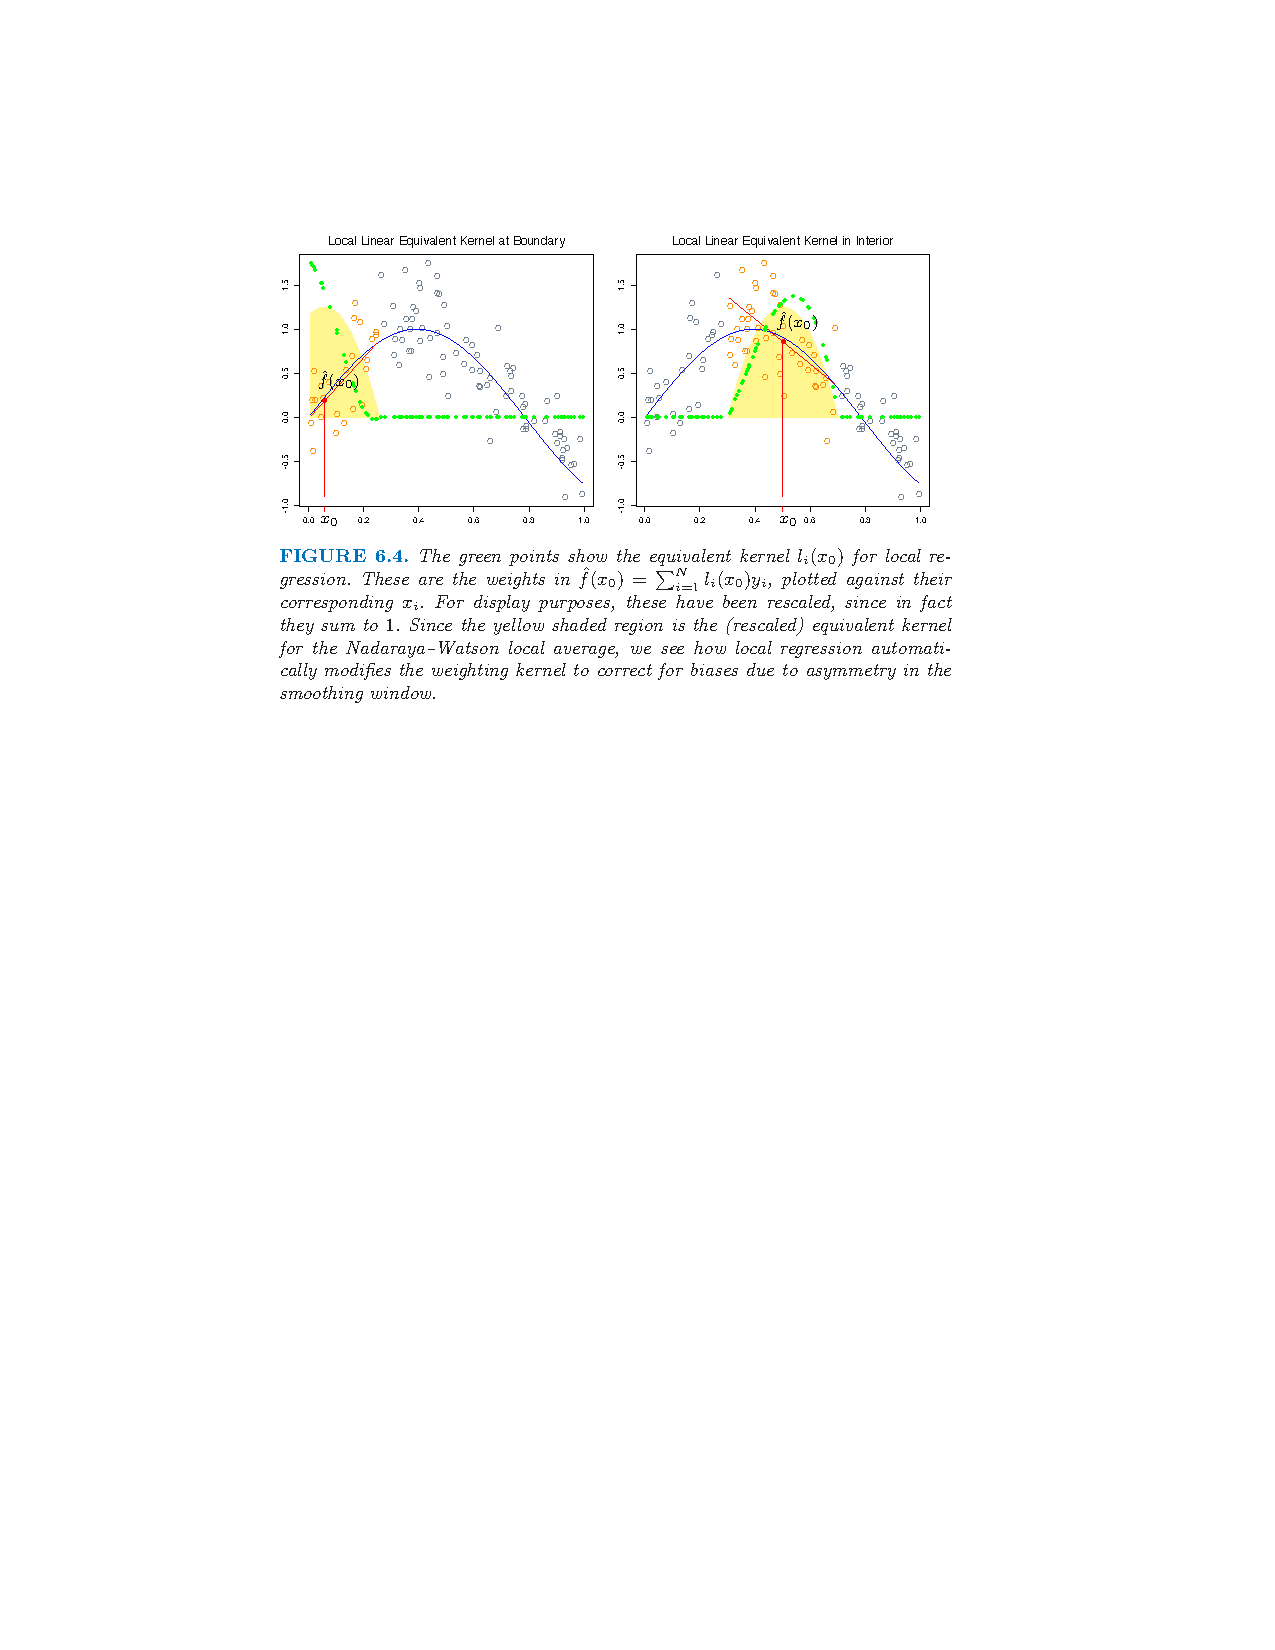
\includegraphics[width=3.5in]{./resources/nwloclinear2.pdf}
\label{loclinear2}
\end{center}
\end{figure}
\end{frame}


 \begin{frame}{Local Quadratic}
\begin{figure}[htbp]
\begin{center}
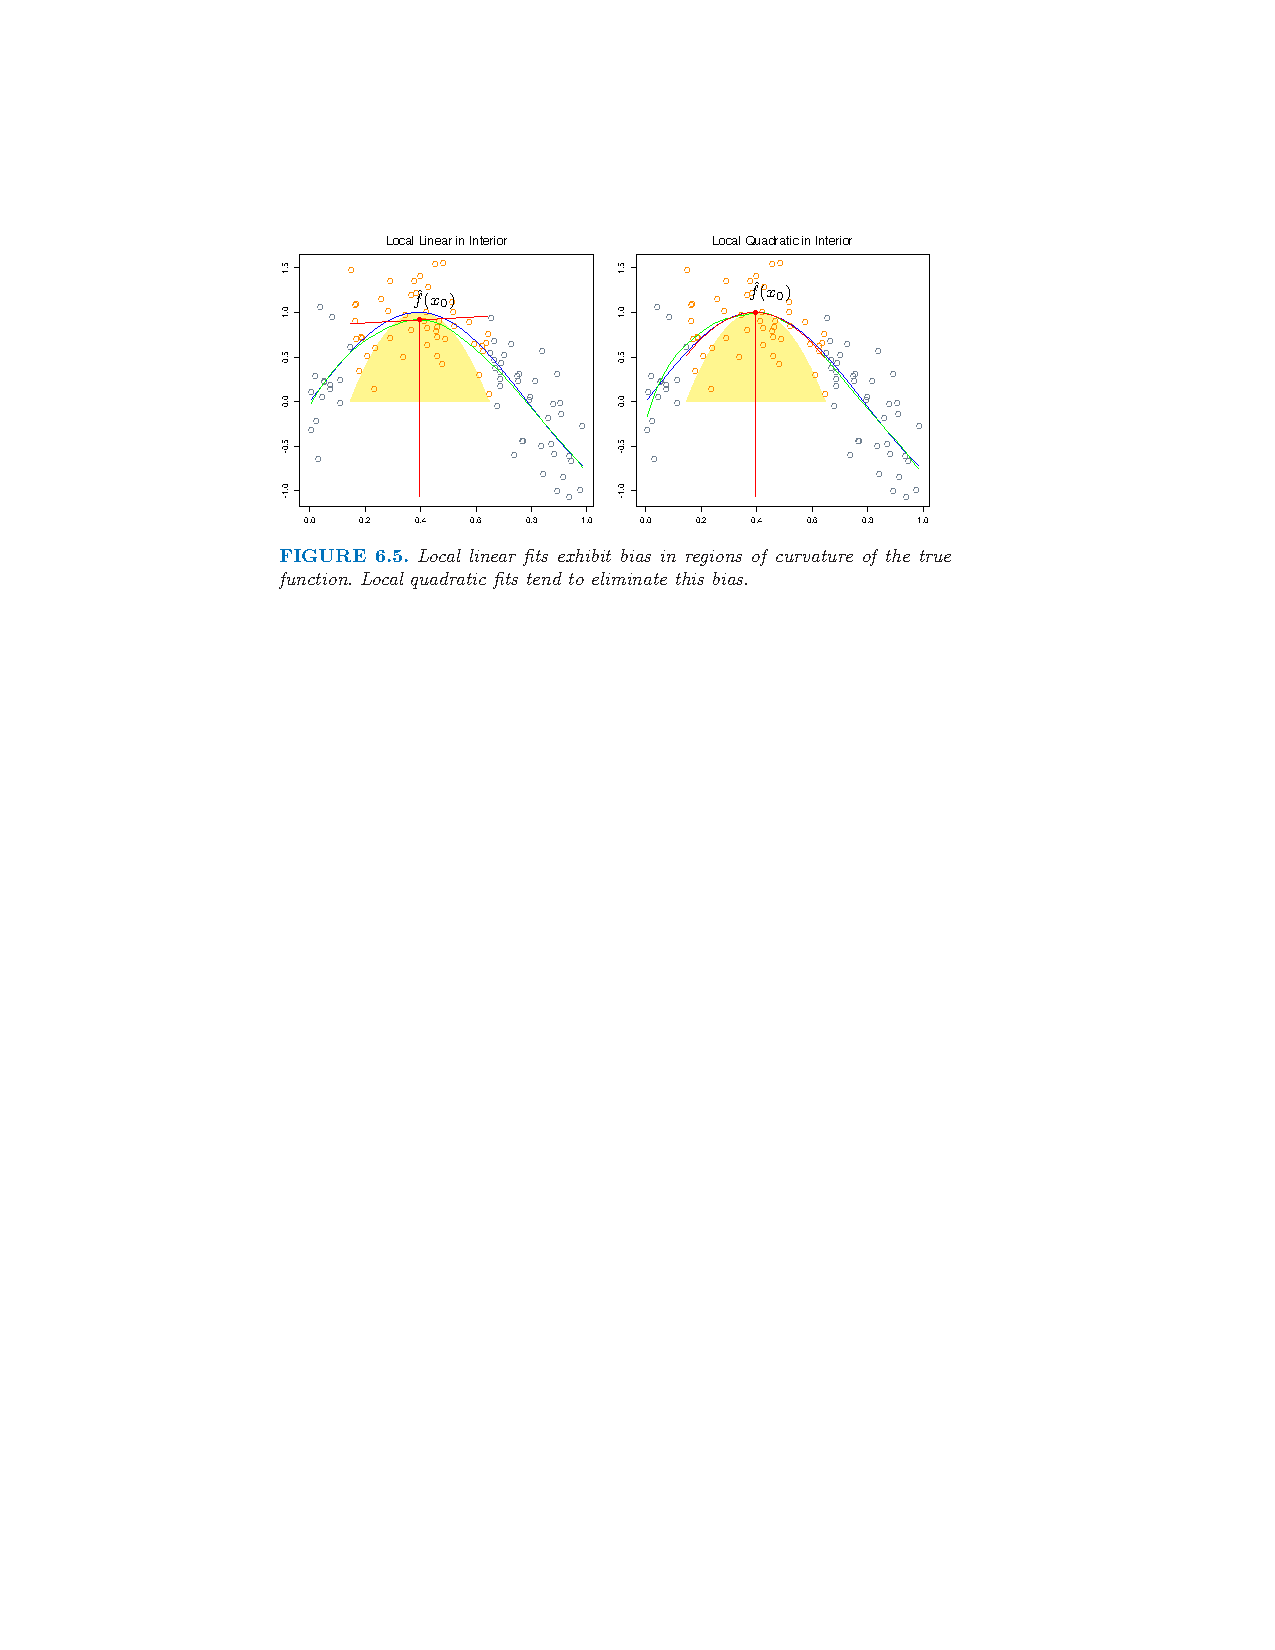
\includegraphics[width=3.5in]{./resources/locquad.pdf}
\label{loclinear2}
\end{center}
\end{figure}
\end{frame}

\frame{\frametitle{Nonparametric Regression, summary, 1}

\pause

Nadaraya--Watson for $E(y\vert x)=m(x)$ 
\[
\hat{m}(x)=\frac{\sum_i y_iK_h(x-x_i)}{\sum_i K_h(x-x_i)}
\]
\begin{itemize}
\item bias in $O(h^2)$, variance in $1/(nh^{p_x})$  
\item optimal $h$ in
$n^{-1/(p+4)}$: then bias, standard error and RMSE all converge at
rate $n^{-2/(p+4)}$
\item to select $h$, no rule of thumb: cross-validate on a subsample and
scale up.
\end{itemize}

}

\frame{\frametitle{Nonparametric Regression, summary, 2}

\pause

Nadaraya--Watson=\textbf{local constant regression}:  to get $\hat{m}(x)$,

\pause

\begin{enumerate}[<+->]
  \item  regress $y_i$ on $1$ with weight $K_h(x-x_i)$
\item take the estimated coeff as your $\hat{m}(x)$.
\end{enumerate}


\pause

Better: \textbf{local linear regression}

\pause

\begin{enumerate}[<+->]
  \item  regress $y_i$ on $1$ and $(x_i-x)$ with weight $K_h(x-x_i)$
\item take the estimated coeffs as your $\hat{m}(x)$ and $\hat{m}^\prime(x)$.
\end{enumerate}

\pause

To estimate the standard errors: bootstrap on an \emph{undersmoothed}
estimate (so that bias is negligible.)
}




\frame{\frametitle{Seminonparametric (=Flexible) Regression}

\pause

{\bf Idea:} we add regressors when we have more data

\pause

$\rightarrow$ \ \textbf{series or sieve estimators}: choose a basis of functions $P_k(x_i)$
($x_i^k$, or orthogonal polynomials, or sines\ldots)

\pause

$\rightarrow$\ run {\em linear regression} $y_i=\sum_{k=1}^M
P_k(x_i)\theta_k+\epsilon_i$

\pause

a reasonable compromise (again, $M$ must go to infinity, more slowly
than $n$).

\pause

Still  curse of dimensionality, and nonparametric asymptotics.


 }
\frame{\frametitle{Splines: trading off fit and smoothness}

\pause

Choose some $0<\lambda<\infty$ and
\[
\min_{m(.)} \sum_i (y_i-m(x_i))^2+\lambda J(m),
\]

\pause

Then we ``obtain'' the
natural cubic spline with knots=$(x_1,\ldots,x_n)$:

\pause

\begin{itemize}[<+->]
\item $m$ is a cubic polynomial between consecutive $x_i$'s
\item it is linear out-of-sample
\item it is $C^2$ everywhere. 
\end{itemize}

\pause

``Consecutive'' implies one-dimensional\ldots harder to generalize to
$p_x>1$.

\pause

\textbf{Orthogonal polynomials:} check out Chebyshev, $1, x,
2x^2-1,4x^3-3x\ldots$ (on $[-1,1]$ here.)
}

\begin{frame}{Review: What was the point?}
\begin{itemize}
\item OLS is lowest variance among linear unbiased estimators.
\item But there are \alert{nonlinear} estimators and potentially \alert{biased} estimators.
\begin{itemize}
\item Everything faces a \alert{bias-variance} tradeoff.
\item Nearly anything can be written as Kernel.
\end{itemize}
\end{itemize}

\end{frame}

%\begin{frame}
%\frametitle{Additive models}
%\pause
%{\em Additive model:} $y=\alpha+\sum_{j=1}^p + f_j (X_j) + +\epsilon$\\
%\pause
%{\em Backfitting algorithm:} start with $\hat{a}=\overline{y}_n$, and some zero--mean
%guesses  $\hat{f}_j \equiv 0 $.
%\pause
%Then for $j=1,\ldots,p,\ldots ,1,2,\ldots,p,\ldots$,
%\pause
%\begin{enumerate}[<+->]
%\item   Define 
%\begin{eqnarray*}
%f_j &\leftarrow& S_j[\{y_i - \hat{\alpha} - \sum_{k\neq j} \hat{f}_k (x_{ik})\}_1^N ]\\
%f_j &\leftarrow&  \hat{f}_j - \frac{1}{N} \sum_{i=1}^N \hat{f}_j (x_{ij}).
%\end{eqnarray*}
%\item Regress $\hat{y}$ on $x_j$ to get $R_j$; then replace $\hat{r}_j$ with $R_j-\frac{1}{n}\sum_i \hat{r}_j(x_{ji})$ (where $S_j$ is some cubic smoothing spline).
%\item Iterate until $\hat{f}_j$ doesn't change.
%\end{enumerate}
%\end{frame}
%


\end{document}